% Options for packages loaded elsewhere
\PassOptionsToPackage{unicode}{hyperref}
\PassOptionsToPackage{hyphens}{url}
%
\documentclass[
  ignorenonframetext,
]{beamer}
\title{Reducción de la factorialidad. Análisis de Componentes
Principales.}
\author{Análisis de Datos curso 2021/2122}
\date{}

\usepackage{pgfpages}
\setbeamertemplate{caption}[numbered]
\setbeamertemplate{caption label separator}{: }
\setbeamercolor{caption name}{fg=normal text.fg}
\beamertemplatenavigationsymbolsempty
% Prevent slide breaks in the middle of a paragraph
\widowpenalties 1 10000
\raggedbottom
\setbeamertemplate{part page}{
  \centering
  \begin{beamercolorbox}[sep=16pt,center]{part title}
    \usebeamerfont{part title}\insertpart\par
  \end{beamercolorbox}
}
\setbeamertemplate{section page}{
  \centering
  \begin{beamercolorbox}[sep=12pt,center]{part title}
    \usebeamerfont{section title}\insertsection\par
  \end{beamercolorbox}
}
\setbeamertemplate{subsection page}{
  \centering
  \begin{beamercolorbox}[sep=8pt,center]{part title}
    \usebeamerfont{subsection title}\insertsubsection\par
  \end{beamercolorbox}
}
\AtBeginPart{
  \frame{\partpage}
}
\AtBeginSection{
  \ifbibliography
  \else
    \frame{\sectionpage}
  \fi
}
\AtBeginSubsection{
  \frame{\subsectionpage}
}
\usepackage{amsmath,amssymb}
\usepackage{lmodern}
\usepackage{iftex}
\ifPDFTeX
  \usepackage[T1]{fontenc}
  \usepackage[utf8]{inputenc}
  \usepackage{textcomp} % provide euro and other symbols
\else % if luatex or xetex
  \usepackage{unicode-math}
  \defaultfontfeatures{Scale=MatchLowercase}
  \defaultfontfeatures[\rmfamily]{Ligatures=TeX,Scale=1}
\fi
\usetheme[]{Rochester}
% Use upquote if available, for straight quotes in verbatim environments
\IfFileExists{upquote.sty}{\usepackage{upquote}}{}
\IfFileExists{microtype.sty}{% use microtype if available
  \usepackage[]{microtype}
  \UseMicrotypeSet[protrusion]{basicmath} % disable protrusion for tt fonts
}{}
\makeatletter
\@ifundefined{KOMAClassName}{% if non-KOMA class
  \IfFileExists{parskip.sty}{%
    \usepackage{parskip}
  }{% else
    \setlength{\parindent}{0pt}
    \setlength{\parskip}{6pt plus 2pt minus 1pt}}
}{% if KOMA class
  \KOMAoptions{parskip=half}}
\makeatother
\usepackage{xcolor}
\IfFileExists{xurl.sty}{\usepackage{xurl}}{} % add URL line breaks if available
\IfFileExists{bookmark.sty}{\usepackage{bookmark}}{\usepackage{hyperref}}
\hypersetup{
  pdftitle={Reducción de la factorialidad. Análisis de Componentes Principales.},
  pdfauthor={Análisis de Datos curso 2021/2122},
  hidelinks,
  pdfcreator={LaTeX via pandoc}}
\urlstyle{same} % disable monospaced font for URLs
\newif\ifbibliography
\usepackage{color}
\usepackage{fancyvrb}
\newcommand{\VerbBar}{|}
\newcommand{\VERB}{\Verb[commandchars=\\\{\}]}
\DefineVerbatimEnvironment{Highlighting}{Verbatim}{commandchars=\\\{\}}
% Add ',fontsize=\small' for more characters per line
\usepackage{framed}
\definecolor{shadecolor}{RGB}{248,248,248}
\newenvironment{Shaded}{\begin{snugshade}}{\end{snugshade}}
\newcommand{\AlertTok}[1]{\textcolor[rgb]{0.94,0.16,0.16}{#1}}
\newcommand{\AnnotationTok}[1]{\textcolor[rgb]{0.56,0.35,0.01}{\textbf{\textit{#1}}}}
\newcommand{\AttributeTok}[1]{\textcolor[rgb]{0.77,0.63,0.00}{#1}}
\newcommand{\BaseNTok}[1]{\textcolor[rgb]{0.00,0.00,0.81}{#1}}
\newcommand{\BuiltInTok}[1]{#1}
\newcommand{\CharTok}[1]{\textcolor[rgb]{0.31,0.60,0.02}{#1}}
\newcommand{\CommentTok}[1]{\textcolor[rgb]{0.56,0.35,0.01}{\textit{#1}}}
\newcommand{\CommentVarTok}[1]{\textcolor[rgb]{0.56,0.35,0.01}{\textbf{\textit{#1}}}}
\newcommand{\ConstantTok}[1]{\textcolor[rgb]{0.00,0.00,0.00}{#1}}
\newcommand{\ControlFlowTok}[1]{\textcolor[rgb]{0.13,0.29,0.53}{\textbf{#1}}}
\newcommand{\DataTypeTok}[1]{\textcolor[rgb]{0.13,0.29,0.53}{#1}}
\newcommand{\DecValTok}[1]{\textcolor[rgb]{0.00,0.00,0.81}{#1}}
\newcommand{\DocumentationTok}[1]{\textcolor[rgb]{0.56,0.35,0.01}{\textbf{\textit{#1}}}}
\newcommand{\ErrorTok}[1]{\textcolor[rgb]{0.64,0.00,0.00}{\textbf{#1}}}
\newcommand{\ExtensionTok}[1]{#1}
\newcommand{\FloatTok}[1]{\textcolor[rgb]{0.00,0.00,0.81}{#1}}
\newcommand{\FunctionTok}[1]{\textcolor[rgb]{0.00,0.00,0.00}{#1}}
\newcommand{\ImportTok}[1]{#1}
\newcommand{\InformationTok}[1]{\textcolor[rgb]{0.56,0.35,0.01}{\textbf{\textit{#1}}}}
\newcommand{\KeywordTok}[1]{\textcolor[rgb]{0.13,0.29,0.53}{\textbf{#1}}}
\newcommand{\NormalTok}[1]{#1}
\newcommand{\OperatorTok}[1]{\textcolor[rgb]{0.81,0.36,0.00}{\textbf{#1}}}
\newcommand{\OtherTok}[1]{\textcolor[rgb]{0.56,0.35,0.01}{#1}}
\newcommand{\PreprocessorTok}[1]{\textcolor[rgb]{0.56,0.35,0.01}{\textit{#1}}}
\newcommand{\RegionMarkerTok}[1]{#1}
\newcommand{\SpecialCharTok}[1]{\textcolor[rgb]{0.00,0.00,0.00}{#1}}
\newcommand{\SpecialStringTok}[1]{\textcolor[rgb]{0.31,0.60,0.02}{#1}}
\newcommand{\StringTok}[1]{\textcolor[rgb]{0.31,0.60,0.02}{#1}}
\newcommand{\VariableTok}[1]{\textcolor[rgb]{0.00,0.00,0.00}{#1}}
\newcommand{\VerbatimStringTok}[1]{\textcolor[rgb]{0.31,0.60,0.02}{#1}}
\newcommand{\WarningTok}[1]{\textcolor[rgb]{0.56,0.35,0.01}{\textbf{\textit{#1}}}}
\usepackage{graphicx}
\makeatletter
\def\maxwidth{\ifdim\Gin@nat@width>\linewidth\linewidth\else\Gin@nat@width\fi}
\def\maxheight{\ifdim\Gin@nat@height>\textheight\textheight\else\Gin@nat@height\fi}
\makeatother
% Scale images if necessary, so that they will not overflow the page
% margins by default, and it is still possible to overwrite the defaults
% using explicit options in \includegraphics[width, height, ...]{}
\setkeys{Gin}{width=\maxwidth,height=\maxheight,keepaspectratio}
% Set default figure placement to htbp
\makeatletter
\def\fps@figure{htbp}
\makeatother
\setlength{\emergencystretch}{3em} % prevent overfull lines
\providecommand{\tightlist}{%
  \setlength{\itemsep}{0pt}\setlength{\parskip}{0pt}}
\setcounter{secnumdepth}{-\maxdimen} % remove section numbering
\usepackage{amsmath,color,array,booktabs,algorithm2e}
\setbeamertemplate{navigation symbols}{}
\setbeamertemplate{footline}[page number]
\newcommand\blue[1]{\textcolor{blue}{#1}}
\newcommand\red[1]{\textcolor{red}{#1}}
\newcommand\green[1]{\textcolor{green}{#1}}
\ifLuaTeX
  \usepackage{selnolig}  % disable illegal ligatures
\fi

\begin{document}
\frame{\titlepage}

\begin{frame}{Introducción}
\protect\hypertarget{introducciuxf3n}{}
\begin{itemize}
\tightlist
\item
  Uno de los problemas centrales del análisis de datos es la
  \red{reducción de la dimensionalidad}.
\item
  Este concepto consiste en describir con cierta precisión los valores
  de las \(p\) variables por un pequeño subconjunto \(r<p\) de ellas con
  una pérdida mínima de información.
\item
  Éste es el objetivo del \red{análisis de componentes principales}:
  dadas \(n\) observaciones de \(p\) variables se analiza,
  \red{si es razonable}, representar esta información en un
  \red{espacio con menos variables}.
\item
  Para alcanzar dicho objetivo, vamos a realizar un
  \red{ajuste ortogonal por mínimos cuadrados}.
\end{itemize}
\end{frame}

\hypertarget{anuxe1lisis-de-componentes-principales}{%
\section{Análisis de Componentes
Principales}\label{anuxe1lisis-de-componentes-principales}}

\begin{frame}{Introducción: Matriz (tabla) de datos.}
\protect\hypertarget{introducciuxf3n-matriz-tabla-de-datos.}{}
\begin{table}
\centering
\begin{tabular}{c|cccc|cc|}
Ind. & $x_1$ & $x_2$ & $\ldots$ & $x_p$ & $v_1$ & $v_2$\\
\hline
$1$      & $x_{11}$ & $x_{12}$ & $\ldots$  & $x_{1p}$ & $v_{11}$ & $v_{12}$ \\
$2$      & $x_{21}$ & $x_{22}$ & $\ldots$  & $x_{2p}$ & $v_{21}$ & $v_{22}$ \\
$3$      & $x_{31}$ & $x_{32}$ & $\ldots$  & $x_{3p}$ & $v_{31}$ & $v_{32}$ \\
$\vdots$ & $\vdots$ & $\vdots$ & $\vdots$  & $\ddots$ & $\vdots$ & $\vdots$ \\
$n$      & $x_{n1}$ & $x_{n2}$ & $\ldots$  & $x_{np}$ & $v_{n1}$ & $v_{n2}$ \\
 \hline
$su_1$   &$su_{11}$ &$su_{12}$ & $\ldots$  &$su_{1p}$ &\multicolumn{2}{|c}{}\\
$su_2$   &$su_{21}$ &$su_{22}$ & $\ldots$  &$su_{2p}$ &\multicolumn{2}{|c}{}\\
\cline{1-5}
\end{tabular}
\end{table}
\end{frame}

\begin{frame}{Introducción: Matriz (tabla) de datos.}
\protect\hypertarget{introducciuxf3n-matriz-tabla-de-datos.-1}{}
\begin{itemize}
\item
  Donde las variables \(x_1,\ldots, x_n\)
  \red{describen una concepto común} de los \(n\) individuos observados.
\item
  Las variables \(v_1\), \(v_2\) \red{son de perfil (o explicativas)} y
  los individuos \(s_1\), \(s_2\) son individuos
  \red{suplementarios o ilustrativos}.
\item
  Tanto los individuos como las variables suplementarias ayudan a
  \red{interpretar la variabilidad de los datos}.
\end{itemize}
\end{frame}

\begin{frame}{Objetivos del análisis}
\protect\hypertarget{objetivos-del-anuxe1lisis}{}
\blue{Objetivos del análisis}

\begin{itemize}
\item
  \red{Reducción de la dimensionalidad} (factorialidad).
\item
  Lo que se busca es un \red{espacio de variables más reducido y fácil
  de interpretar}.
\item
  El problema es que si reducimos el número de variables es posible que
  \red{perdamos parte toda la variabilidad de los datos originales}.
\item
  Así la idea básica es
  \red{consentir una pérdida de información para lograr una
  ganancia en la significación}.
\end{itemize}
\end{frame}

\begin{frame}{Análisis Factorial}
\protect\hypertarget{anuxe1lisis-factorial}{}
\begin{itemize}
\tightlist
\item
  Algunos autores consideran el \red{ACP como una parte del Análisis
  Factorial}.
\item
  En las \red{técnicas de Análisi Factorial} se postula que
  \red{la variabilidad total} se puede explicar mediante distintos tipos
  de factores:
\item
  \red{factores comunes} subyacentes (\(F_i\)).
\item
  \red{factores específicos} de las variables (\(E_i\)).
\item
  \red{Error o fluctuaciones aleatorias} (\(A_i\)).
\end{itemize}

\[X_1=\alpha_{1 1} F_1+ \alpha_{1 2} F_2+\cdots +\alpha_{1 k} F_k+ E_1+ A_1\]
\[X_2=\alpha_{2 1} F_1+ \alpha_{2 2} F_2+\cdots +\alpha_{2 k} F_k+ E_2+ A_2\]
\[\cdots\cdots\cdots\cdots\cdots\cdots\cdots\cdots\cdots\cdots\cdots\cdots\]
\[X_p=\alpha_{p 1} F_1+ \alpha_{p 2} F_2+\cdots +\alpha_{p k} F_k+ E_p+ A_p\]
\end{frame}

\begin{frame}{Análisis Factorial}
\protect\hypertarget{anuxe1lisis-factorial-1}{}
\begin{itemize}
\tightlist
\item
  Podríamos decir que en un Análisis Factorial se fija a priori la
  cantidad de varianza de cada variable que debe quedar interpretada por
  los factores comunes.
\item
  Este valor recibe el nombre de comunalidad y se suele representar como
  \(h_i^2\).
\end{itemize}

Utilizaremos las siguientes notaciones:

\begin{itemize}
\tightlist
\item
  La comunalidad de la variable \(X_i\),\(h_i^2\), es la varianza
  explicada por \(F_1,F_2,\ldots F_k.\)
\item
  La diferencia \(s_i^2-h_i^2\) es la varianza de la variable \(X_i\)
  que explican los factores específicos y aleatorios.
\end{itemize}

\[\color{red}{\mbox{Var. observada = Var. común + Var. específica y aleatorios}}.\]
\end{frame}

\hypertarget{el-problema-de-los-componentes-principales}{%
\section{El problema de los Componentes
Principales}\label{el-problema-de-los-componentes-principales}}

\begin{frame}{El problema de los Componentes Principales}
\protect\hypertarget{el-problema-de-los-componentes-principales-1}{}
\red{Todos los factores son comunes}

\[X_1=\alpha_{1 1} CP_1+ \alpha_{1 2} CP_2+\cdots +\alpha_{1 p} CP_p\]
\[X_2=\alpha_{2 1} CP_1+ \alpha_{2 2} CP_2+\cdots +\alpha_{2 p} CP_p\]
\[\cdots\cdots\cdots\cdots\cdots\cdots\cdots\cdots\cdots\cdots\cdots\cdots\]
\[X_p=\alpha_{p 1} CP_1+ \alpha_{p 2} CP_2+\cdots +\alpha_{p p} CP_p\]

Se trata de encontrar unas nuevas variables \(CP_1,\ldots CP_p\), a las
que llamaremos componentes principales, de forma que:
\end{frame}

\begin{frame}{El problema de los Componentes Principales}
\protect\hypertarget{el-problema-de-los-componentes-principales-2}{}
\begin{itemize}
\tightlist
\item
  Se cumplan las condiciones anteriores.
\item
  El origen de las variables esté situado en el vector de medias o
  centro de gravedad de las observaciones.
\item
  Sean incorreladas entre si \(Cor(CP_i,CP_j)=0\) para
  \(i\not= j, i,j =1,\ldots,p\).
\item
  Se cumple que \(Var(CP_1)\geq Var(CP_2)\geq\cdots\geq Var(CP_p)\) y
  hagan máximas estas varianzas.
\item
  Se conserva la varianza total (inercia) de la nube de puntos.
\end{itemize}
\end{frame}

\hypertarget{tipos-de-a.c.p.}{%
\section{Tipos de A.C.P.}\label{tipos-de-a.c.p.}}

\begin{frame}{Tipos de A.C.P:}
\protect\hypertarget{tipos-de-a.c.p}{}
\begin{itemize}
\tightlist
\item
  Sobre los datos centrados: a cada variable se le resta su media
  \(x_i-\overline{x}_i\);
  \red{en estas notas solo consideraremos este caso}.
\item
  Sobre los datos tipificados \(\frac{x_{i}-\overline{x}_i}{s_i}\).
\item
  En el primer caso las variables centradas tienen media cero y la misma
  varianza que las variables originales: se le suele llamar ACP de
  covarianzas.
\item
  En el segundo caso las variables tipificadas tienen media cero y
  varianza 1: se le suele llamar ACP de correlaciones o normado.
\end{itemize}
\end{frame}

\begin{frame}{Tipos de A.C.P:}
\protect\hypertarget{tipos-de-a.c.p-1}{}
Recordemos que dada una matriz de datos \(\mathbf{X}\) (\(n\times p\) es
decir de \(n\) individuos y \(p\) variables) representábamos por
\(\tilde{\mathbf{X}}\) la matriz de datos centrada. Entonces:

\begin{itemize}
\tightlist
\item
  La matriz de covarianzas de \(\mathbf{X}\) viene dada por
\end{itemize}

\[\mathbf{S}=1/n \tilde{\mathbf{X}}^t\tilde{\mathbf{X}}\]

\begin{itemize}
\tightlist
\item
  Si llamamos \(\mathbf{Z}\) a la tabla de los datos tipificados, la
  matriz de correlaciones viene dada por
\end{itemize}

\[\mathbf{R}=1/n \mathbf{Z}^t\mathbf{Z}\]
\end{frame}

\begin{frame}{A.C.P propiedades}
\protect\hypertarget{a.c.p-propiedades}{}
\blue{Propiedades}

\begin{itemize}
\tightlist
\item
  Los
  \red{componentes principales vienen determinadas por los vectores propios ortonormales}
  (ordenados de mayor a menor valor propio) de la matriz de covarianzas
  (para datos centrados) y de la matriz de correlaciones (para los datos
  tipificados).
\item
  Así en el ACP de covarianzas cada variable interviene con su propia
  varianza mientras que el ACP de correlaciones todas las variables
  tienen varianza 1.
\end{itemize}
\end{frame}

\begin{frame}{A.C.P: interpretación geométrica}
\protect\hypertarget{a.c.p-interpretaciuxf3n-geomuxe9trica}{}
Supongamos que \(p=2\) y que la \red{nube de puntos} de nuestra tabla de
datos es la de la siguiente figura:

\begin{center}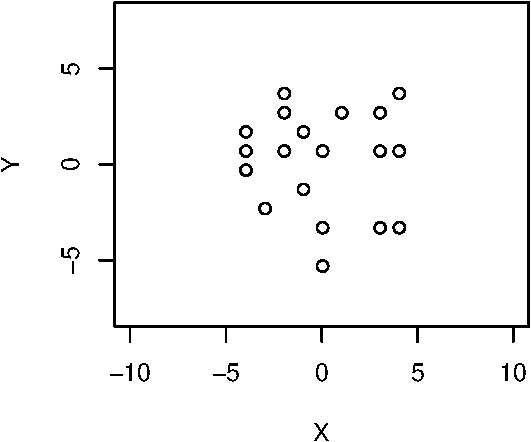
\includegraphics{AnalisisComponentesPrincipales_fusion_files/figure-beamer/inter_geom1-1} \end{center}
\end{frame}

\begin{frame}{Interpretación geométrica}
\protect\hypertarget{interpretaciuxf3n-geomuxe9trica}{}
La siguiente figura muestra las dos \red{componentes principales}, es
decir, las direcciones de las proyecciones que tienen máxima
variabilidad.

\begin{center}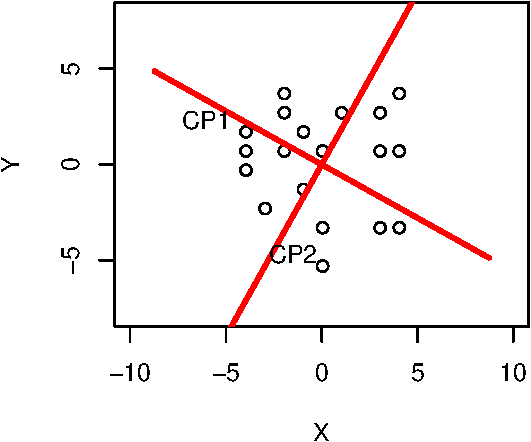
\includegraphics{AnalisisComponentesPrincipales_fusion_files/figure-beamer/inter2-1} \end{center}
\end{frame}

\begin{frame}{Interpretación geométrica}
\protect\hypertarget{interpretaciuxf3n-geomuxe9trica-1}{}
Si projectamos en la dirección de la \red{primera componente},
obtendremos las proyecciones siguientes (en \blue{azul}):

\begin{center}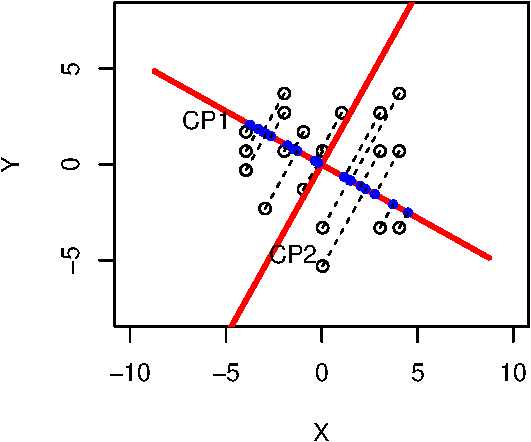
\includegraphics{AnalisisComponentesPrincipales_fusion_files/figure-beamer/inter3-1} \end{center}
\end{frame}

\begin{frame}{Interpretación geométrica}
\protect\hypertarget{interpretaciuxf3n-geomuxe9trica-2}{}
Lo que significa que la varianza de los puntos azules es máxima; en el
sentido de que cualquier otra dirección o recta las proyecciones sobre
ésta tendrán´n a lo más igual varianza. \medskip

Los puntos azules representan las coordenadas que tienen los puntos de
nuestra tabla de datos (centrada) tomando como eje de abcisas el
\red{primer componente} \(CP_1\).
\end{frame}

\begin{frame}{Interpretación geométrica}
\protect\hypertarget{interpretaciuxf3n-geomuxe9trica-3}{}
Si projectamos en la dirección del \red{segundo componente}, obtendremos
las proyecciones siguientes (en \green{verde}):

\begin{center}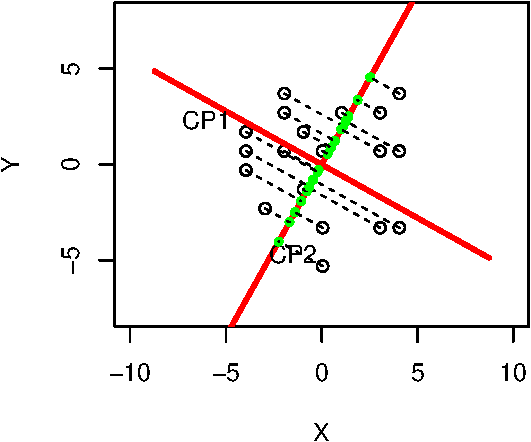
\includegraphics{AnalisisComponentesPrincipales_fusion_files/figure-beamer/inter4.1-1} \end{center}
\end{frame}

\hypertarget{acp-covarianzas}{%
\section{ACP covarianzas:}\label{acp-covarianzas}}

\begin{frame}{ACP covarianzas:}
\protect\hypertarget{acp-covarianzas-1}{}
\begin{itemize}
\tightlist
\item
  Sea \(\mathbf{S}\) la matriz de covarianzas de orden \(p\). Calculamos
  sus valores propios
\end{itemize}

\[\lambda_1\geq \lambda_2\geq\ldots\geq\lambda_p\]

y los correspondientes vectores propios ortonormales (perpendiculares y
de norma 1)

\[\mathbf{u}_1,\mathbf{u}_2,\ldots,\mathbf{u}_p\]

\begin{itemize}
\item
  Las \red{direcciones de los componentes principales} quedan
  determinadas por su respectivo vector propio.
\item
  \red{Cálculo de las coordenadas de la nueva matriz de datos respecto
  a las nuevas variables $CP$:}

  \[\mathbf{CP}= \tilde{\mathbf{X}} \mathbf{u},\] donde \(\mathbf{u}\)
  es la matriz de los vectores propios.
\end{itemize}
\end{frame}

\begin{frame}{Ejemplo}
\protect\hypertarget{ejemplo}{}
Vamos a realizar un ACP sobre el ejemplo de la estatura de un niño
recién nacido.

\begin{table}
\centering
\begin{tabular}{|c|c|c|c|c|}\hline
$x_1$ & $x_2$ & $x_3$ & $x_4$&Sexo\\
\hline
78&48.2&2.75&29.5& Niña\\
69&45.5&2.15&26.3& Niña\\
77&46.3&4.41&32.2& Niña\\
88&49&5.52&36.5& Niño\\
67&43&3.21&27.2& Niña\\
80&48&4.32&27.7& Niña\\
74&48&2.31&28.3& Niña\\
94&53&4.3&30.3& Niño\\
102&58&3.71&28.7& Niño
\\
\hline
\end{tabular}
\end{table}
\end{frame}

\begin{frame}{Ejemplo}
\protect\hypertarget{ejemplo-1}{}
Donde:

\begin{itemize}
\tightlist
\item
  \(x_1:\) edad en días
\item
  \(x_2:\) estatura al nacer en cm.
\item
  \(x_3:\) peso en Kg. al nacer
\item
  \(x_4:\) aumento en tanto por ciento de su peso con respecto de su
  peso al nacer.
\item
  El sexo es una variable de perfil que podría ayudarnos a explicar
  algunos de los resultados del análisis de componentes principales.
\end{itemize}
\end{frame}

\begin{frame}[fragile]{Código para la carga de datos}
\protect\hypertarget{cuxf3digo-para-la-carga-de-datos}{}
\begin{Shaded}
\begin{Highlighting}[]
\NormalTok{n }\OtherTok{=} \DecValTok{9}
\NormalTok{p }\OtherTok{=} \DecValTok{4}
\NormalTok{X }\OtherTok{=} \FunctionTok{matrix}\NormalTok{(}\FunctionTok{c}\NormalTok{(}\DecValTok{78}\NormalTok{,}\FloatTok{48.2}\NormalTok{,}\FloatTok{2.75}\NormalTok{,}\FloatTok{29.5}\NormalTok{,}\DecValTok{69}\NormalTok{,}\FloatTok{45.5}\NormalTok{,}\FloatTok{2.15}\NormalTok{,}\FloatTok{26.3}\NormalTok{,}
\DecValTok{77}\NormalTok{,}\FloatTok{46.3}\NormalTok{,}\FloatTok{4.41}\NormalTok{,}\FloatTok{32.2}\NormalTok{, }\DecValTok{88}\NormalTok{,}\DecValTok{49}\NormalTok{,}\FloatTok{5.52}\NormalTok{,}\FloatTok{36.5}\NormalTok{, }\DecValTok{67}\NormalTok{,}\DecValTok{43}\NormalTok{,}\FloatTok{3.21}\NormalTok{,}\FloatTok{27.2}\NormalTok{,}
\DecValTok{80}\NormalTok{,}\DecValTok{48}\NormalTok{,}\FloatTok{4.32}\NormalTok{,}\FloatTok{27.7}\NormalTok{, }\DecValTok{74}\NormalTok{,}\DecValTok{48}\NormalTok{,}\FloatTok{2.31}\NormalTok{,}\FloatTok{28.3}\NormalTok{, }\DecValTok{94}\NormalTok{,}\DecValTok{53}\NormalTok{,}\FloatTok{4.3}\NormalTok{,}\FloatTok{30.3}\NormalTok{,}
\DecValTok{102}\NormalTok{,}\DecValTok{58}\NormalTok{,}\FloatTok{3.71}\NormalTok{,}\FloatTok{28.7}\NormalTok{),}\AttributeTok{nrow=}\NormalTok{n,}\AttributeTok{byrow=}\NormalTok{T)}
\NormalTok{Datos}\OtherTok{=} \FunctionTok{as.data.frame}\NormalTok{(X)}
\FunctionTok{names}\NormalTok{(Datos) }\OtherTok{=} \FunctionTok{paste}\NormalTok{(}\StringTok{"x"}\NormalTok{,}\FunctionTok{c}\NormalTok{(}\DecValTok{1}\SpecialCharTok{:}\NormalTok{p),}\AttributeTok{sep=}\StringTok{""}\NormalTok{)}
\NormalTok{Sexo }\OtherTok{=} \FunctionTok{as.factor}\NormalTok{(}\FunctionTok{c}\NormalTok{(}\StringTok{"Niña"}\NormalTok{,}\StringTok{"Niña"}\NormalTok{,}\StringTok{"Niña"}\NormalTok{,}\StringTok{"Niño"}\NormalTok{,}
\StringTok{"Niña"}\NormalTok{,}\StringTok{"Niña"}\NormalTok{,}\StringTok{"Niña"}\NormalTok{,}\StringTok{"Niño"}\NormalTok{,}\StringTok{"Niño"}\NormalTok{))}
\NormalTok{Datos}\SpecialCharTok{$}\NormalTok{Sexo}\OtherTok{=}\NormalTok{Sexo}
\end{Highlighting}
\end{Shaded}
\end{frame}

\begin{frame}[fragile]{Código diagrama matricial}
\protect\hypertarget{cuxf3digo-diagrama-matricial}{}
El siguiente código dibuja un diagrama matricial de las variables.

\begin{Shaded}
\begin{Highlighting}[]
\FunctionTok{pairs}\NormalTok{(Datos[,}\DecValTok{1}\SpecialCharTok{:}\DecValTok{4}\NormalTok{],}\AttributeTok{pch=}\DecValTok{21}\NormalTok{,}
\AttributeTok{bg =} \FunctionTok{c}\NormalTok{(}\StringTok{"red"}\NormalTok{, }\StringTok{"blue"}\NormalTok{)[}\FunctionTok{unclass}\NormalTok{(Datos}\SpecialCharTok{$}\NormalTok{Sexo)],}
\AttributeTok{main=}\StringTok{"Diagrama matricial de las variables.}
\SpecialCharTok{\textbackslash{}n}\StringTok{ Azul Niño, Rojo Niña"}\NormalTok{)}
\FunctionTok{legend}\NormalTok{(}\DecValTok{15}\NormalTok{,}\SpecialCharTok{{-}}\DecValTok{4}\NormalTok{,}\AttributeTok{legend=}\FunctionTok{levels}\NormalTok{(Datos}\SpecialCharTok{$}\NormalTok{Sexo),}\AttributeTok{pch=}\DecValTok{21}\NormalTok{,}
\AttributeTok{pt.bg=}\FunctionTok{c}\NormalTok{(}\StringTok{"red"}\NormalTok{, }\StringTok{"blue"}\NormalTok{),}\AttributeTok{title=}\StringTok{"Sexo"}\NormalTok{)}
\end{Highlighting}
\end{Shaded}

que producen este gráfico\ldots{}
\end{frame}

\begin{frame}{Diagrama matricial}
\protect\hypertarget{diagrama-matricial}{}
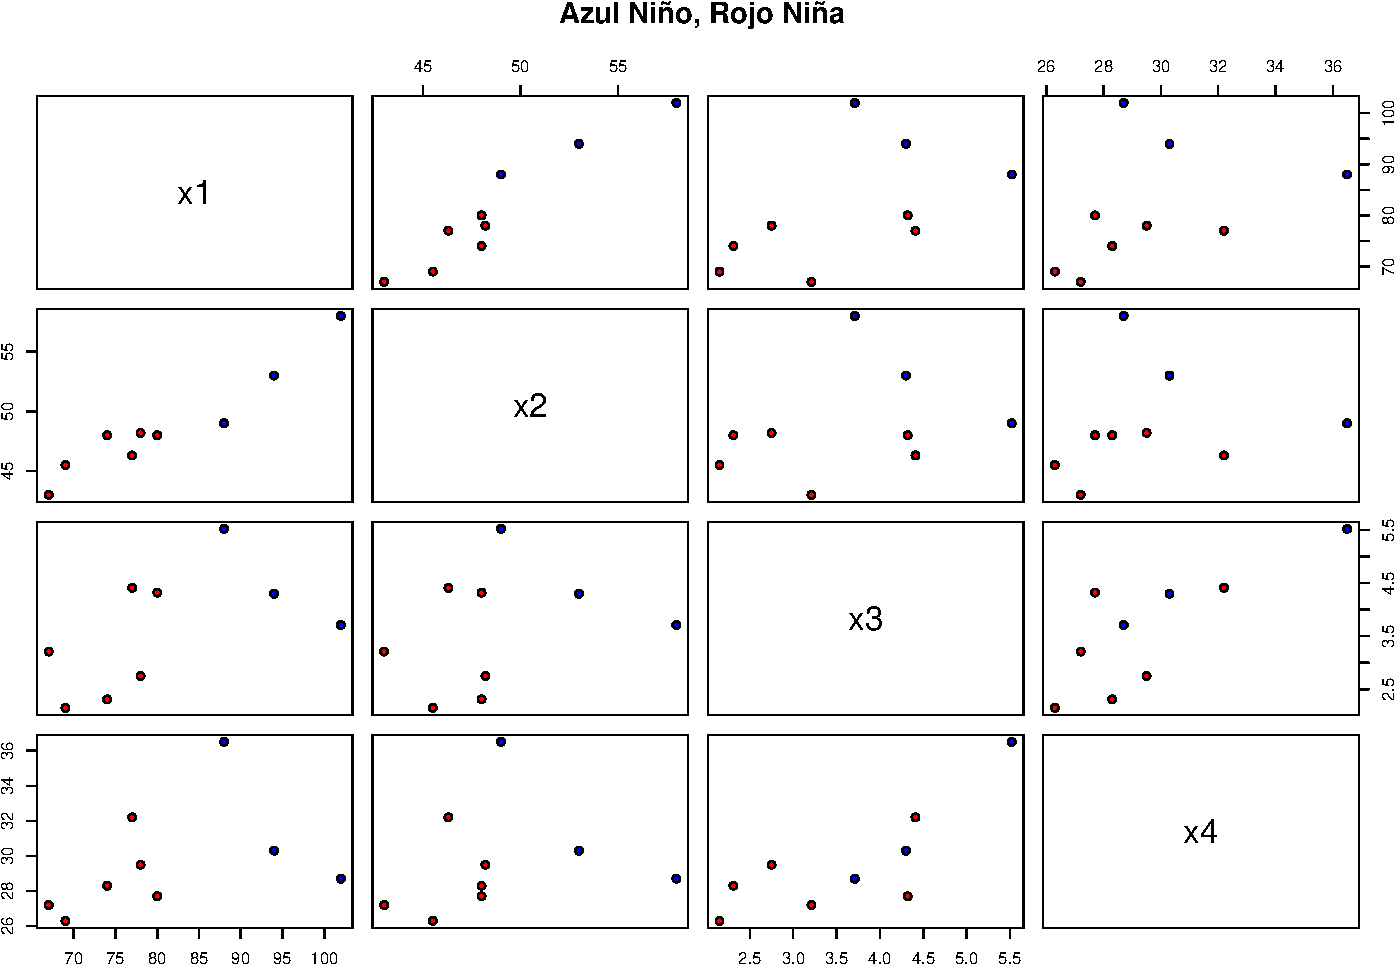
\includegraphics{AnalisisComponentesPrincipales_fusion_files/figure-beamer/unnamed-chunk-2-1.pdf}
\end{frame}

\begin{frame}{Cálculos básicos}
\protect\hypertarget{cuxe1lculos-buxe1sicos}{}
En lo que sigue todos los datos se redondean al tercer decimal.

Daremos el código de R que realiza el cálculo, en el código no se
redondea: La matriz centrada de los datos anteriores es:

\[
\tilde{\mathbf{X}}=
\left(
\begin{array}{rrrr}
-3.000 & -0.578 & -0.881 & -0.133 \\
-12.000 & -3.278 & -1.481 & -3.333 \\
-4.000 & -2.478 & 0.779 & 2.567 \\
7.000 & 0.222 & 1.889 & 6.867 \\
-14.000 & -5.778 & -0.421 & -2.433 \\
-1.000 & -0.778 & 0.689 & -1.933 \\
-7.000 & -0.778 & -1.321 & -1.333 \\
13.000 & 4.222 & 0.669 & 0.667 \\
21.000 & 9.222 & 0.079 & -0.933
\end{array}
\right)
\]
\end{frame}

\begin{frame}[fragile]{Cálculos básicos}
\protect\hypertarget{cuxe1lculos-buxe1sicos-1}{}
\begin{Shaded}
\begin{Highlighting}[]
\FunctionTok{colMeans}\NormalTok{(X)}
\end{Highlighting}
\end{Shaded}

\begin{verbatim}
## [1] 81.000000 48.777778  3.631111 29.633333
\end{verbatim}

\begin{Shaded}
\begin{Highlighting}[]
\NormalTok{n}\OtherTok{=}\FunctionTok{dim}\NormalTok{(X)[}\DecValTok{1}\NormalTok{]}
\NormalTok{n}
\end{Highlighting}
\end{Shaded}

\begin{verbatim}
## [1] 9
\end{verbatim}

\begin{Shaded}
\begin{Highlighting}[]
\NormalTok{Hn}\OtherTok{=}\FunctionTok{diag}\NormalTok{(}\FunctionTok{rep}\NormalTok{(}\DecValTok{1}\NormalTok{,n))}\SpecialCharTok{{-}}\DecValTok{1}\SpecialCharTok{/}\NormalTok{n}\CommentTok{\# matriz centralizadora}
\FunctionTok{dim}\NormalTok{(Hn)}
\end{Highlighting}
\end{Shaded}

\begin{verbatim}
## [1] 9 9
\end{verbatim}
\end{frame}

\begin{frame}[fragile]{Cálculos básicos}
\protect\hypertarget{cuxe1lculos-buxe1sicos-2}{}
\begin{Shaded}
\begin{Highlighting}[]
\CommentTok{\# filas 1 a 9 y columnas 1 a 4 }
\CommentTok{\# de la matriz centralizadora}
\FunctionTok{round}\NormalTok{(Hn[}\DecValTok{1}\SpecialCharTok{:}\DecValTok{9}\NormalTok{,}\DecValTok{1}\SpecialCharTok{:}\DecValTok{4}\NormalTok{],}\DecValTok{4}\NormalTok{)}
\end{Highlighting}
\end{Shaded}

\begin{verbatim}
##          [,1]    [,2]    [,3]    [,4]
##  [1,]  0.8889 -0.1111 -0.1111 -0.1111
##  [2,] -0.1111  0.8889 -0.1111 -0.1111
##  [3,] -0.1111 -0.1111  0.8889 -0.1111
##  [4,] -0.1111 -0.1111 -0.1111  0.8889
##  [5,] -0.1111 -0.1111 -0.1111 -0.1111
##  [6,] -0.1111 -0.1111 -0.1111 -0.1111
##  [7,] -0.1111 -0.1111 -0.1111 -0.1111
##  [8,] -0.1111 -0.1111 -0.1111 -0.1111
##  [9,] -0.1111 -0.1111 -0.1111 -0.1111
\end{verbatim}
\end{frame}

\begin{frame}[fragile]{Cálculos básicos}
\protect\hypertarget{cuxe1lculos-buxe1sicos-3}{}
\begin{Shaded}
\begin{Highlighting}[]
\NormalTok{cX}\OtherTok{=}\NormalTok{Hn}\SpecialCharTok{\%*\%}\NormalTok{X }\CommentTok{\# matriz centrada cálculo matricial}
\FunctionTok{round}\NormalTok{(cX,}\DecValTok{3}\NormalTok{)}
\end{Highlighting}
\end{Shaded}

\begin{verbatim}
##       [,1]   [,2]   [,3]   [,4]
##  [1,]   -3 -0.578 -0.881 -0.133
##  [2,]  -12 -3.278 -1.481 -3.333
##  [3,]   -4 -2.478  0.779  2.567
##  [4,]    7  0.222  1.889  6.867
##  [5,]  -14 -5.778 -0.421 -2.433
##  [6,]   -1 -0.778  0.689 -1.933
##  [7,]   -7 -0.778 -1.321 -1.333
##  [8,]   13  4.222  0.669  0.667
##  [9,]   21  9.222  0.079 -0.933
\end{verbatim}
\end{frame}

\begin{frame}{Ejemplo}
\protect\hypertarget{ejemplo-2}{}
\begin{itemize}
\tightlist
\item
  La matriz de covarianzas de los datos anteriores es:
\end{itemize}

\[
\mathbf{S}=
\begin{pmatrix}
119.333 & 43.133 & 6.148 & 12.511 \\
 43.133 & 17.193 & 1.148 & 1.886 \\
 6.148 & 1.148 & 1.111 & 2.428 \\
 12.511 & 1.886 & 2.428 & 8.624 
\end{pmatrix}
\]

\begin{itemize}
\tightlist
\item
  Los valores propios son:
\end{itemize}

\[\lambda_1=136.615,\quad \lambda_2=8.861,\quad \lambda_3 = 0.738,\quad \lambda_4 = 0.047.\]
\end{frame}

\begin{frame}{Ejemplo}
\protect\hypertarget{ejemplo-3}{}
\begin{itemize}
\tightlist
\item
  Los vectores propios ortonormales correspondientes a los valores
  propios, son las columnas de la siguiente matriz:
\end{itemize}

\[
\left(
\begin{array}{rrrr}
0.934 & -0.022 & 0.256 & 0.247 \\
0.339 & 0.354 & -0.661 & -0.568 \\
0.047 & -0.248 & 0.566 & -0.785 \\
0.097 & -0.902 & -0.421 & -0.013
\end{array}
\right)
\]
\end{frame}

\begin{frame}[fragile]{Ejemplo}
\protect\hypertarget{ejemplo-4}{}
\begin{verbatim}
##            [,1]      [,2]     [,3]      [,4]
## [1,] 119.333333 43.133333 6.147778 12.511111
## [2,]  43.133333 17.192840 1.147802  1.886296
## [3,]   6.147778  1.147802 1.110610  2.427852
## [4,]  12.511111  1.886296 2.427852  8.624444
\end{verbatim}

\begin{verbatim}
## eigen() decomposition
## $values
## [1] 136.61529623   8.86125966   0.73789460   0.04677667
## 
## $vectors
##            [,1]        [,2]       [,3]        [,4]
## [1,] 0.93439437 -0.02238785  0.2555755  0.24715806
## [2,] 0.33947477  0.35413519 -0.6610845 -0.56772562
## [3,] 0.04701065 -0.24770838  0.5656945 -0.78512437
## [4,] 0.09723192 -0.90151407 -0.4214714 -0.01342527
\end{verbatim}
\end{frame}

\begin{frame}{Ejemplo}
\protect\hypertarget{ejemplo-5}{}
\begin{itemize}
\tightlist
\item
  Las expresiones de las variables nuevas \(CP_i\) en función de las
  antiguas, notemos que se calculan sobre los datos centrados, son:
\end{itemize}

\[
\begin{array}{rl}
CP_1 = & 0.934\cdot \tilde{X}_1 + 0.339\cdot \tilde{X}_2 + 0.047\cdot
\tilde{X}_3\\ & + 0.097 \cdot \tilde{X}_4, \\
CP_2 = & -0.022\cdot \tilde{X}_1 +0.354\cdot \tilde{X}_2 -0.248 \cdot
\tilde{X}_3 \\ & -0.902 \cdot \tilde{X}_4, \\
CP_3 = & 0.256\cdot \tilde{X}_1 -0.661 \cdot \tilde{X}_2 +0.566\cdot \tilde{X}_3
\\ &-0.421\cdot \tilde{X}_4, \\
CP_4 = & 0.247 \cdot \tilde{X}_1 - 0.568\cdot \tilde{X}_2 - 0.785\cdot
\tilde{X}_3 \\ & - 0.013 \cdot \tilde{X}_4.
\end{array}
\]
\end{frame}

\begin{frame}{Ejemplo}
\protect\hypertarget{ejemplo-6}{}
\begin{itemize}
\tightlist
\item
  La nueva matriz de datos respecto de las nuevas variables será:
\end{itemize}

\[
\mathbf{CP}= \tilde{\mathbf{X}} \mathbf{u} =
\left(
\begin{array}{rrrr}
-3.054 & 0.201 & -0.827 & 0.280 \\
-12.719 & 2.480 & -0.333 & 0.103 \\
-4.293 & -3.295 & -0.025 & -0.228 \\
7.373 & -6.736 & -0.183 & 0.029 \\
-15.299 & 0.565 & 1.029 & 0.183 \\
-1.354 & 1.319 & 1.463 & -0.321 \\
-6.997 & 1.411 & -1.460 & -0.233 \\
13.677 & 0.437 & 0.629 & 0.282 \\
22.666 & 3.618 & -0.292 & -0.095 \\
\end{array}
\right)
\]
\end{frame}

\begin{frame}[fragile]{Ejemplo}
\protect\hypertarget{ejemplo-7}{}
\begin{itemize}
\tightlist
\item
  Se puede observar que si se multiplican escalarmente dos columnas
  cualesquiera, el resultado es nulo. Es decir, las columnas de la nueva
  matriz de datos son ortogonales dos a dos.
\end{itemize}

\begin{verbatim}
##             [,1]       [,2]        [,3]        [,4]
##  [1,]  -3.053710  0.2010126 -0.82701014  0.28011692
##  [2,] -12.719190  2.4798083 -0.33296991  0.10258907
##  [3,]  -4.292542 -3.2947403 -0.02544479 -0.22791715
##  [4,]   7.372657 -6.7363084 -0.18344827  0.02874558
##  [5,] -15.299325  0.5653125  1.02890237  0.18327243
##  [6,]  -1.354027  1.3192330  1.46314663 -0.32050161
##  [7,]  -6.996545  1.4105455 -1.46023526 -0.23340514
##  [8,]  13.676731  0.4374966  0.62864176  0.28187987
##  [9,]  22.665952  3.6176402 -0.29158239 -0.09477995
\end{verbatim}
\end{frame}

\begin{frame}{Ejemplo}
\protect\hypertarget{ejemplo-8}{}
Como podemos observar, nuestro análisis que interpretado por la variable
de perfil sexo ya que distingue entre niños y niñas con las dos primeras
componentes.

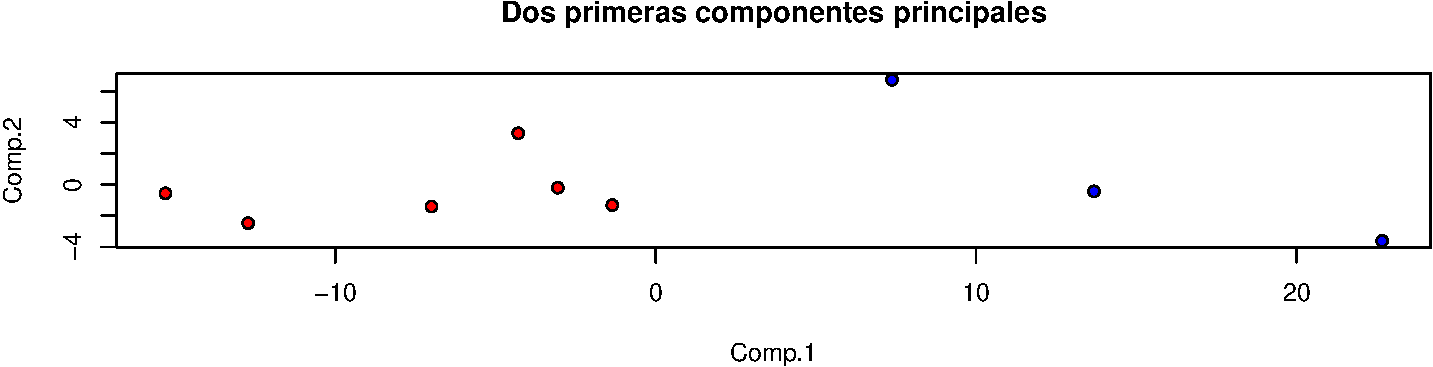
\includegraphics{AnalisisComponentesPrincipales_fusion_files/figure-beamer/plotACP1-1.pdf}
\end{frame}

\begin{frame}[fragile]{Ejemplo}
\protect\hypertarget{ejemplo-9}{}
El siguiente código dibuja todos los componentes

\begin{Shaded}
\begin{Highlighting}[]
\FunctionTok{pairs}\NormalTok{(solacp}\SpecialCharTok{$}\NormalTok{scores,}\AttributeTok{pch=}\DecValTok{21}\NormalTok{,}
\AttributeTok{bg =} \FunctionTok{c}\NormalTok{(}\StringTok{"red"}\NormalTok{, }\StringTok{"blue"}\NormalTok{)[}\FunctionTok{unclass}\NormalTok{(Datos}\SpecialCharTok{$}\NormalTok{Sexo)],}
\AttributeTok{main=}\StringTok{"Diagrama matricial de }
\StringTok{los componentes principales"}\NormalTok{)}
\end{Highlighting}
\end{Shaded}
\end{frame}

\begin{frame}{Ejemplo}
\protect\hypertarget{ejemplo-10}{}
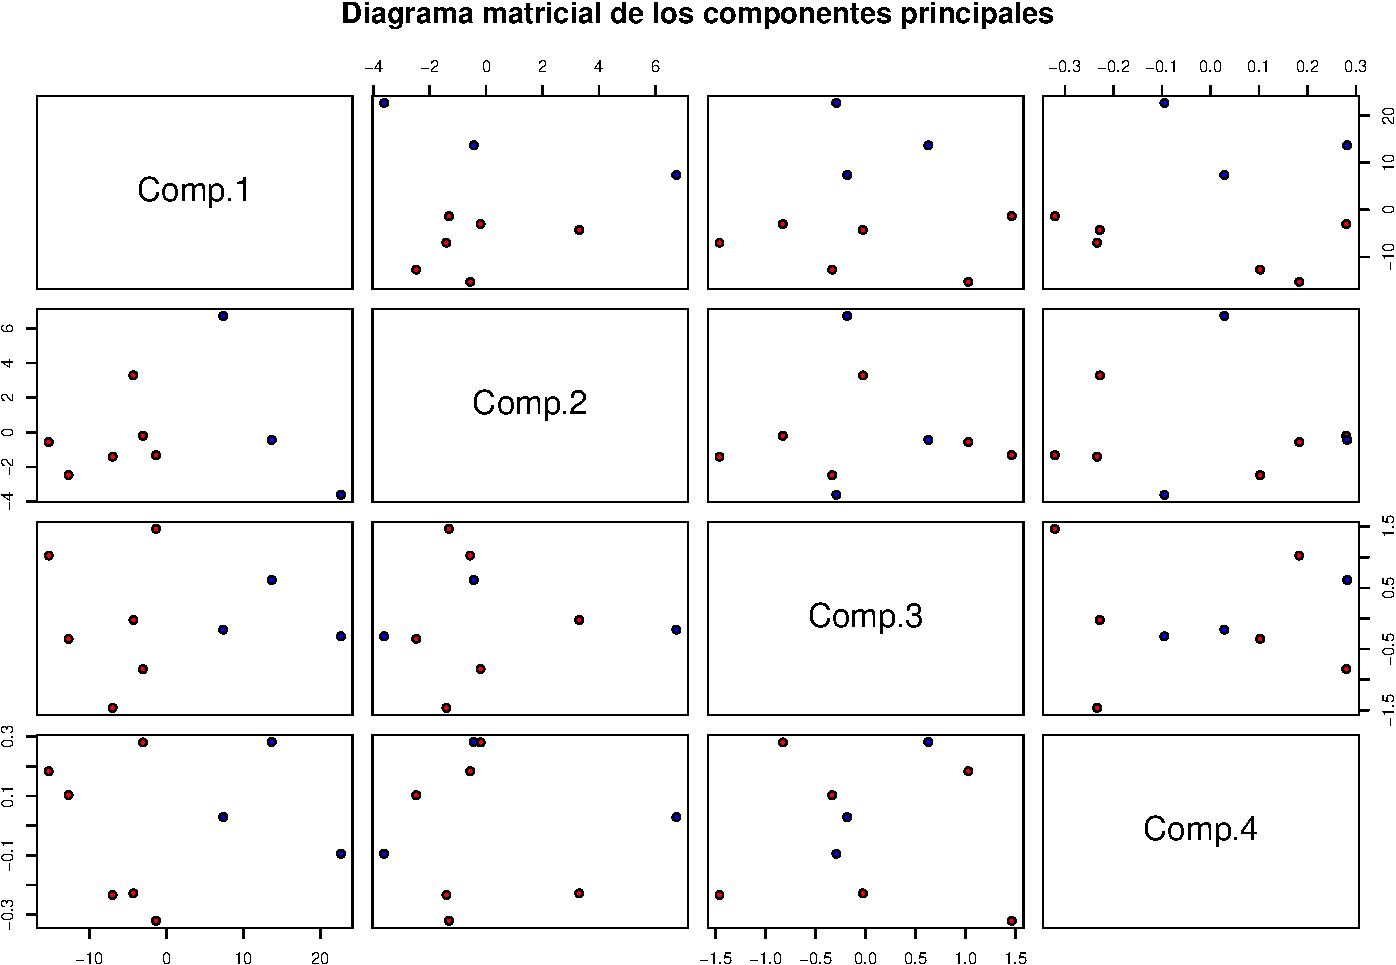
\includegraphics{AnalisisComponentesPrincipales_fusion_files/figure-beamer/pairsacptodos1-1.pdf}
\end{frame}

\hypertarget{acp-correlaciones.}{%
\section{ACP correlaciones.}\label{acp-correlaciones.}}

\begin{frame}{ACP correlaciones.}
\protect\hypertarget{acp-correlaciones.-1}{}
Sea \(\mathbf{R}\) la matriz de correlaciones de orden \(p\).
Calcularemos sus valores propios

\[\lambda_1\geq \lambda_2\geq\ldots\geq\lambda_p.\]

y los correspondientes vectores propios ortonormales.

\[\mathbf{u}_1,\mathbf{u}_2,\ldots,\mathbf{u}_p.\]

Las direcciones de los componentes principales quedan determinadas por
el vector propio correspondiente.
\end{frame}

\begin{frame}{ACP correlaciones.}
\protect\hypertarget{acp-correlaciones.-2}{}
\blue{Cálculo de las coordenadas de la nueva matriz de datos respecto de las
nuevas variables $CP$:} \[\mathbf{CP}= \mathbf{Z} \mathbf{u},\] donde
\(Z\) es la matriz de datos tipificados y \(\mathbf{u}\) es la matriz de
los vectores propios.
\end{frame}

\begin{frame}{Ejemplo}
\protect\hypertarget{ejemplo-11}{}
\begin{itemize}
\tightlist
\item
  Realicemos un análisis ACP de correlaciones con el ejemplo anterior.
\item
  La matriz tipificada de datos es: \[
  \mathbf{Z}=
  \left(
  \begin{array}{rrrr}
  -0.275 & -0.139 & -0.836 & -0.045 \\
   -1.099 & -0.791 & -1.405 & -1.135 \\
   -0.366 & -0.598 & 0.739 & 0.874 \\
   0.641 & 0.054 & 1.792 & 2.338 \\
   -1.282 & -1.393 & -0.400 & -0.829 \\
   -0.092 & -0.188 & 0.654 & -0.658 \\
   -0.641 & -0.188 & -1.254 & -0.454 \\
   1.190 & 1.018 & 0.635 & 0.227 \\
   1.922 & 2.224 & 0.075 & -0.318 
  \end{array}
  \right)
  \]
\end{itemize}
\end{frame}

\begin{frame}{Ejemplo}
\protect\hypertarget{ejemplo-12}{}
\begin{itemize}
\tightlist
\item
  La matriz de correlaciones \(\mathbf{R}\) vale, en este caso: \[
  \mathbf{R} =
  \left(
  \begin{array}{rrrr}
  1.000 & 0.952 & 0.534 & 0.390 \\
  0.952 & 1.000 & 0.263 & 0.155 \\
  0.534 & 0.263 & 1.000 & 0.784 \\
  0.390 & 0.155 & 0.784 & 1.000 
  \end{array}
  \right)
  \]
\item
  Los valores propios de dicha matriz son: \[
  2.560,\quad 1.229,\quad 0.208,\quad 0.00325.
  \]
\item
  La matriz de los vectores propios es: \[
  \left(
  \begin{array}{rrrr}
  0.573 & 0.359 & -0.038 & 0.736 \\
  0.478 & 0.578 & 0.145 & -0.646 \\
  0.499 & -0.459 & -0.707 & -0.201 \\
  0.442 & -0.572 & 0.691 & -0.029 
  \end{array}
  \right)
  \]
\end{itemize}
\end{frame}

\begin{frame}{Ejemplo}
\protect\hypertarget{ejemplo-13}{}
\begin{itemize}
\tightlist
\item
  Las expresiones de las variables nuevas \(CP_i\) en función de las
  antiguas \(Z_i\)son:
\end{itemize}

\[
\begin{array}{rl}
CP_1 = & 0.573\cdot Z_1 +0.478\cdot Z_2 +0.499\cdot Z_3\\ & +0.442 \cdot Z_4,
\\
CP_2 = & 0.359\cdot Z_1 + 0.578\cdot Z_2 -0.459 \cdot Z_3 \\ & -0.572 \cdot Z_4,
\\
CP_3 = & -0.038\cdot Z_1 +0.145 \cdot Z_2 -0.707\cdot Z_3 \\ &+0.691\cdot Z_4,
\\
CP_4 = & 0.736 \cdot Z_1 - 0.646\cdot Z_2 - 0.201\cdot Z_3 \\ & - 0.029 \cdot
Z_4.
\end{array}
\]
\end{frame}

\begin{frame}{Ejemplo}
\protect\hypertarget{ejemplo-14}{}
\begin{itemize}
\tightlist
\item
  La nueva matriz de datos respecto de las nuevas variables será:
\end{itemize}

\[
\mathbf{CP} = \mathbf{Z} \mathbf{u} =
\begin{pmatrix}
-0.661 & 0.231 & 0.550 & 0.057 \\
 -2.209 & 0.443 & 0.137 & 0.018 \\
 0.259 & -1.316 & 0.008 & -0.058 \\
 2.319 & -1.899 & 0.332 & 0.008 \\
 -1.965 & -0.608 & -0.444 & 0.061 \\
 -0.107 & -0.065 & -0.941 & -0.058 \\
 -1.282 & 0.497 & 0.570 & -0.085 \\
 1.585 & 0.594 & -0.189 & 0.084 \\
 2.061 & 2.122 & -0.023 & -0.027 
\end{pmatrix}
\]

\begin{itemize}
\tightlist
\item
  Se puede observar que si calculamos el producto escalar de dos
  columnas cualesquiera, es resultado es nulo. Es decir, las columnas de
  la nueva matriz de datos son ortogonales dos a dos.
\end{itemize}
\end{frame}

\hypertarget{propiedades-acp-covarianzas.}{%
\section{Propiedades ACP
covarianzas.}\label{propiedades-acp-covarianzas.}}

\begin{frame}{Propiedades ACP covarianzas.}
\protect\hypertarget{propiedades-acp-covarianzas.-1}{}
Sea \(\mathbf{X}\) una matriz de datos \(n\times p\) y sea

\[
\mathbf{S}=\begin{pmatrix}
s_1^2& s_{ 1 2}&\ldots &s_{1 p}\\
s_{2 1}& s_{2}^2&\ldots &s_{2 p}\\
\vdots & \vdots &\ddots & \vdots\\
s_{p 1}& s_{ p 2}&\ldots &s_{p}^2
\end{pmatrix}
\] su matriz de covarianzas.

Recordemos que \(s_i^2\) es la varianza de la variable \(\mathbf{x}_i\)
y que \(s_{i j}\) son las covarianzas de la variables \(\mathbf{x}_i\) y
\(\mathbf{x}_j\).

Además la \(\mbox{Varianza Total}= tr(\mathbf{S})=\sum_{i=1}^p s_i^2\)
\end{frame}

\begin{frame}{Propiedades ACP covarianzas.}
\protect\hypertarget{propiedades-acp-covarianzas.-2}{}
\begin{itemize}
\tightlist
\item
  \(Var(\mathbf{CP}_i)= \lambda_i\). La varianza de cada componente
  principal es su valor propio.
\item
  \(\sum_{i=1}^n Var(\mathbf{CP}_i)=\sum_{i=1}^n \lambda_i=tr(\mathbf{S})=\sum_{i=1}^n s_i^2\).
  Por lo tanto los componentes principales reproducen la varianza total
\item
  Los componentes principales tienen correlación cero entre sí (son
  \emph{incorrelados}) por lo tanto su matriz de covarianzas es
  \[\mathbf{S}_{CP}=\left(\begin{array}{cccc}
  \lambda_1& 0 &\ldots &0\\
  0& \lambda_{2}&\ldots & 0\\
  \vdots & \vdots & & \vdots\\
  0 & 0&\ldots &\lambda_{p}
  \end{array}
  \right)\]
\end{itemize}
\end{frame}

\begin{frame}{Propiedades ACP covarianzas.}
\protect\hypertarget{propiedades-acp-covarianzas.-3}{}
\begin{itemize}
\item
  \(\det(\mathbf{S}_{CP})=\prod_{i=1}^n \lambda_i =\det(\mathbf{S})\).
  Luego los componentes principales conservan la varianza generalizada.
\item
  La proporción de varianza explicada por la componente \(j\)-ésima es
  \[\frac{\lambda_j}{\sum_{i=1}^n \lambda_i}.\]
\end{itemize}

Además al ser* incorrelados* la proporción de varianza explicada por los
\(k\) primeros componentes es \[\frac{\sum_{i=1}^k
\lambda_i}{\sum_{i=1}^n \lambda_i}.\]

\begin{itemize}
\tightlist
\item
  \(\mbox{Cov}(\tilde{\mathbf{X}}_i, \mathbf{CP}_j)=\lambda_j u_{j i}\);
  \(corr(\tilde{\mathbf{X}}_i, \mathbf{CP}_j)=\frac{\sqrt{\lambda_j} u_{j i}}{s_i}\)
  donde \(u_{j i}\) es la \(i\)-ésima componente del vector propio
  \(\mathbf{u}_j\).
\end{itemize}
\end{frame}

\begin{frame}{Ejemplo}
\protect\hypertarget{ejemplo-15}{}
Vamos a comprobar las propiedades anteriores con nuestro ejemplo.
Recordemos las matrices de datos de las variables originales
\(\mathbf{X}\) (centradas) y de las variables en componentes principales
\(\mathbf{CP}\): \[
{\tiny 
\begin{array}{rl}
\tilde{\mathbf{X}} =& 
\left(
\begin{array}{rrrr}
-3.000 & -0.578 & -0.881 & -0.133 \\
 -12.000 & -3.278 & -1.481 & -3.333 \\
 -4.000 & -2.478 & 0.779 & 2.567 \\
 7.000 & 0.222 & 1.889 & 6.867 \\
 -14.000 & -5.778 & -0.421 & -2.433 \\
 -1.000 & -0.778 & 0.689 & -1.933 \\
 -7.000 & -0.778 & -1.321 & -1.333 \\
 13.000 & 4.222 & 0.669 & 0.667 \\
 21.000 & 9.222 & 0.079 & -0.933 
\end{array}
\right) ,
\\ &\\
\mathbf{CP}= &
\left(
\begin{array}{rrrr}
-3.054 & 0.201 & -0.827 & 0.280 \\
 -12.719 & 2.480 & -0.333 & 0.103 \\
 -4.293 & -3.295 & -0.025 & -0.228 \\
 7.373 & -6.736 & -0.183 & 0.029 \\
 -15.299 & 0.565 & 1.029 & 0.183 \\
 -1.354 & 1.319 & 1.463 & -0.321 \\
 -6.997 & 1.411 & -1.460 & -0.233 \\
 13.677 & 0.437 & 0.629 & 0.282 \\
 22.666 & 3.618 & -0.292 & -0.095 
\end{array}
\right).
\end{array}}
\]
\end{frame}

\begin{frame}{Ejemplo}
\protect\hypertarget{ejemplo-16}{}
\begin{itemize}
\item
  La matriz de los vectores propios de la matriz \(\mathbf{S}\) era: \[
  {\tiny 
  \left(
  \begin{array}{rrrr}
  0.934 & -0.022 & 0.256 & 0.247 \\
   0.339 & 0.354 & -0.661 & -0.568 \\
   0.047 & -0.248 & 0.566 & -0.785 \\
   0.097 & -0.902 & -0.421 & -0.013 
  \end{array}\right).}
  \]
\item
  Las varianzas de las variables \(CP\) son las siguientes: \[
  \begin{array}{llcll}
  \mbox{Var}(\mathbf{CP}_1) & =136.615,\ & \mbox{Var}(\mathbf{CP}_2) & =8.861,\\ 
  \mbox{Var}(\mathbf{CP}_3) & =0.738,\ &\mbox{Var}(\mathbf{CP}_4) & =0.0468,
  \end{array}
  \] que \red{son los valores propios de la matriz de
  covarianzas $\mathbf{S}$}.
\item
  La \red{traza de la matriz $\mathbf{S}$} vale:
  \(tr(\mathbf{S})=146.261\). Si sumamos los 4 valores propios, su valor
  \textbackslash red\{coincide con la suma de los valores propios:
  \[\lambda_1+\lambda_2+\lambda_3+\lambda_4 = 146.261.\]
\end{itemize}
\end{frame}

\begin{frame}{Ejemplo}
\protect\hypertarget{ejemplo-17}{}
\begin{itemize}
\tightlist
\item
  La \red{matriz de covarianzas de las variables $\mathbf{CP}$} es:
\end{itemize}

\[
cov(\mathbf{CP})=
\left(
\begin{array}{rrrr}
136.615 & 0.000 & 0.000 & 0.000 \\
 0.000 & 8.861 & 0.000 & 0.000 \\
 0.000 & 0.000 & 0.738 & 0.000 \\
 0.000 & 0.000 & 0.000 & 0.047 
\end{array}
\right)
\]

Podemos observar que es una matriz diagonal con los valores propios de
la matriz \(\mathbf{S}\) en la diagonal.

\begin{itemize}
\tightlist
\item
  El
  \red{determinante de las matrices de covarianzas de $\tilde{\mathbf{X}}$}
  y \(\mathbf{CP}\) vale \(41.785\), valor que
  \red{coincide con el producto de los valores
  propios de la matriz $\mathbf{S}$}: \[
  \prod_{i=1}^4 \lambda_i= 136.615\cdot 8.861\cdot 0.738\cdot 0.0468 = 41.785.
  \]
\end{itemize}
\end{frame}

\begin{frame}{Ejemplo}
\protect\hypertarget{ejemplo-18}{}
La proporción de varianza explicada por los componentes es:

\begin{tabular}{|l|l|}\hline
Variables&Varianza Explicada\\\hline
$\mathbf{CP}_1$&$136.615/146.261=0.934$\\\hline
$\mathbf{CP}_{1,2}$&$(136.615+8.861)/146.261=0.995$\\\hline
$\mathbf{CP}_{1,2,3}$&$(136.615+8.861+0.738)/146.261=0.999$\\\hline
$\mathbf{CP}_{1,2,3,4}$&$1$\\\hline
\end{tabular}
\end{frame}

\begin{frame}{Ejemplo}
\protect\hypertarget{ejemplo-19}{}
\begin{itemize}
\tightlist
\item
  La matriz de covarianzas entre las variables \(\tilde{\mathbf{X}}\) y
  \(\mathbf{CP}\) vale: \[
  cov(\tilde{\mathbf{X}},\mathbf{CP})=
  \left(
  \begin{array}{rrrr}
  127.653 & -0.198 & 0.189 & 0.012 \\
   46.377 & 3.138 & -0.488 & -0.027 \\
   6.422 & -2.195 & 0.417 & -0.037 \\
   13.283 & -7.989 & -0.311 & -0.001 
  \end{array}
  \right)
  \]
\end{itemize}

Recuperemos la matriz de vectores propios de la matriz \(\mathbf{S}\):

\[
{\tiny \left(
\begin{array}{rrrr}
0.934 & -0.022 & 0.256 & 0.247 \\
 0.339 & 0.354 & -0.661 & -0.568 \\
 0.047 & -0.248 & 0.566 & -0.785 \\
 0.097 & -0.902 & -0.421 & -0.013 
\end{array}
\right)
.}
\]
\end{frame}

\begin{frame}{Ejemplo}
\protect\hypertarget{ejemplo-20}{}
Si multiplicamos la primera columna de la matriz anterior

\[
\begin{pmatrix}
0.934\\ 0.339\\ 0.047\\ 0.097
\end{pmatrix}
\]

por el valor propio \(136.615\) de la matriz \(\mathbf{S}\) obtenemos la
primera columna de la matriz

\(\mbox{Cov}(\tilde{\mathbf{X}},\mathbf{CP})\):

\[
136.615\cdot \begin{pmatrix}0.934\\ 0.339\\ 0.047\\ 0.097\end{pmatrix}=
\begin{pmatrix}
127.652 \\ 46.377 \\ 6.422 \\ 13.283
\end{pmatrix}
\]
\end{frame}

\begin{frame}{Ejemplo}
\protect\hypertarget{ejemplo-21}{}
\begin{itemize}
\tightlist
\item
  En general, tenemos que
\end{itemize}

\[
\mathbf{u}\cdot \mbox{diag}(\lambda) = \mbox{Cov}(\tilde{\mathbf{X}},\mathbf{CP}),
\]

donde \(\mathbf{u}\) es la matriz formada por los vectores propios de la
matriz \(\mathbf{S}\) y \(\mbox{diag}(\lambda)\) es una matriz diagonal
con los valores propios de la matriz \(\mathbf{S}\) en la diagonal.
\end{frame}

\begin{frame}{Propiedades ACP covarianzas.}
\protect\hypertarget{propiedades-acp-covarianzas.-4}{}
\begin{itemize}
\item
  La \red{primer componente principal} es la recta que \red{conserva
  mayor inercia} de la nube de puntos.
\item
  Las \red{dos primeras componentes} principales forman el \red{plano}
  que conserva \red{mayor inercia} de la nube de puntos.
\item
  Lo mismo sucede con los espacios formados por las \(k\) primeras
  componentes
\end{itemize}
\end{frame}

\hypertarget{propiedades-acp-correlaciones.}{%
\section{Propiedades ACP
correlaciones.}\label{propiedades-acp-correlaciones.}}

\begin{frame}{Propiedades ACP correlaciones.}
\protect\hypertarget{propiedades-acp-correlaciones.-1}{}
Sea \(\mathbf{X}\) una matriz de datos \(n\times p\) y sea

\[\mathbf{R}=\left(\begin{array}{cccc}
1& r_{ 1 2}&\ldots &r_{1 p}\\
r_{2 1}& 1&\ldots &r_{2 p}\\
\vdots & \vdots & \ddots& \vdots\\
r_{p 1}& s_{ p 2}&\ldots &1
\end{array}
\right)\] Su matriz de correlaciones. Se verifican las siguientes
propiedades:
\end{frame}

\begin{frame}{Propiedades ACP correlaciones}
\protect\hypertarget{propiedades-acp-correlaciones}{}
\begin{itemize}
\item
  Recordemos que la diagonal es \(1\) pues es la varianza de los datos
  tipificados y que \(r_{i j}\) son las correlaciones lineales de la
  variables \(\mathbf{x}_i\) y \(\mathbf{x}_j\).
\item
  Además la \(\mbox{Varianza Total}= tr(\mathbf{R})=p\)
\item
  \(Var(\mathbf{CP}_i)= \lambda_i\). El valor propio del componente es
  igual a su varianza
\item
  \(\sum_{i=1}^n var(\mathbf{CP}_i)=\sum_{i=1}^n \lambda_i=tr(\mathbf{R})=p\).
  Por lo tanto los componentes principales reproducen la varianza total
  y ésta es igual al numero de variables \(p\).
\end{itemize}
\end{frame}

\begin{frame}{Propiedades ACP correlaciones.}
\protect\hypertarget{propiedades-acp-correlaciones.-2}{}
\begin{itemize}
\tightlist
\item
  Los componentes principales tienen correlación cero entre sí (son
  \emph{incorrelados}) por lo tanto su matriz de covarianzas ( que este
  caso es igual a la de correlaciones es
\end{itemize}

\[\mathbf{S}_{CP}=\left(\begin{array}{cccc}
\lambda_1& 0 &\ldots &0\\
0& \lambda_{2}&\ldots & 0\\
\vdots & \vdots &\ddots & \vdots\\
0 & 0&\ldots &\lambda_{p}
\end{array}
\right)\]
\end{frame}

\begin{frame}{Propiedades ACP correlaciones.}
\protect\hypertarget{propiedades-acp-correlaciones.-3}{}
\begin{itemize}
\item
  \(\det(\mathbf{S}_{CP})=\prod_{i=1}^n \lambda_i =\det(\mathbf{R})\).
  Luego los componentes principales conservan la varianza generalizada.
\item
  La proporción de varianza explicada por cada componente es
  \[\frac{\lambda_i}{p}.\]
\end{itemize}

Además al ser \emph{incorreladas} la proporción de varianza explicada
por los \(k\) primeros componentes es
\[\frac{\sum_{i=1}^k \lambda_i}{p}.\]

\begin{itemize}
\tightlist
\item
  \(corr(\mathbf{Z}_i, \mathbf{CP}_j)=\sqrt{\lambda_j}\cdot u_{j i}\)
  donde \(u_{j i}\) es la \(i\)-ésima componente del vector propio
  \(\mathbf{u}_j\).
\end{itemize}
\end{frame}

\begin{frame}{Propiedades ACP correlaciones.}
\protect\hypertarget{propiedades-acp-correlaciones.-4}{}
Vamos a comprobar las propiedades anteriores con nuestro ejemplo.
Recordemos las matrices de datos estandarizada\(\mathbf{Z}\)y de las
variables en componentes principales \(\mathbf{CP}\):

\[
\mathbf{Z}=
\begin{pmatrix}
-0.275 & -0.139 & -0.836 & -0.045 \\
 -1.099 & -0.791 & -1.405 & -1.135 \\
 -0.366 & -0.598 & 0.739 & 0.874 \\
 0.641 & 0.054 & 1.792 & 2.338 \\
 -1.282 & -1.393 & -0.400 & -0.829 \\
 -0.092 & -0.188 & 0.654 & -0.658 \\
 -0.641 & -0.188 & -1.254 & -0.454 \\
 1.190 & 1.018 & 0.635 & 0.227 \\
 1.922 & 2.224 & 0.075 & -0.318 
\end{pmatrix}
\]
\end{frame}

\begin{frame}{Ejemplo}
\protect\hypertarget{ejemplo-22}{}
\[
\mathbf{CP}=
\begin{pmatrix}
-0.661 & 0.231 & 0.550 & 0.057 \\
 -2.209 & 0.443 & 0.137 & 0.018 \\
 0.259 & -1.316 & 0.008 & -0.058 \\
 2.319 & -1.899 & 0.332 & 0.008 \\
 -1.965 & -0.608 & -0.444 & 0.061 \\
 -0.107 & -0.065 & -0.941 & -0.058 \\
 -1.282 & 0.497 & 0.570 & -0.085 \\
 1.585 & 0.594 & -0.189 & 0.084 \\
 2.061 & 2.122 & -0.023 & -0.027 
\end{pmatrix}.
\]
\end{frame}

\begin{frame}{Ejemplo}
\protect\hypertarget{ejemplo-23}{}
\red{Las varianzas de las variables}
\(\textcolor{red}{\mathbf{CP}_i=\lambda_{i}}\) son las siguientes:

\[
\begin{array}{llcll}
\mbox{Var}(\mathbf{CP}_1) & =2.560,\ & \mbox{Var}(\mathbf{CP}_2) & =1.229,\\
\mbox{Var}(\mathbf{CP}_3) & =0.208,\ & \mbox{Var}(\mathbf{CP}_4) & =0.00325,
\end{array}
\]

Estos valores son los
\textcolor{red}{valores propios de la matriz $\mathbf{R}$}.
\end{frame}

\begin{frame}{Ejemplo}
\protect\hypertarget{ejemplo-24}{}
Se puede comprobar que su
\textcolor{red}{suma vale $4$, que es el valor de $p$} en nuestro caso.

Si calculamos la \textcolor{red}{matriz de covarianzas de las variables}
\(\textcolor{red}{\mathbf{CP}}\) obtenemos una
\textcolor{red}{matriz diagonal} que son los valores propios de la
matriz \(\mathbf{R}\) calculados anteriormente:

\[
\mbox{Cov}(\mathbf{CP})= \mathbf{S}_{\mathbf{CP}} = 
\begin{pmatrix}
2.560 & 0.000 & 0.000 & 0.000 \\
 0.000 & 1.229 & 0.000 & 0.000 \\
 0.000 & 0.000 & 0.208 & 0.000 \\
 0.000 & 0.000 & 0.000 & 0.003 
\end{pmatrix},
\]
\end{frame}

\begin{frame}{Ejemplo}
\protect\hypertarget{ejemplo-25}{}
\textcolor{red}{El determinante de la matriz}
\(\textcolor{red}{\mathbf{S}_{\mathbf{CP}}}\) \textcolor{red}{ es:}

\[\textcolor{red}{\det(\mathbf{S}_{\mathbf{CP}})=0.00213},\]

que coincide con el \textcolor{red}{producto de los
valores propios de la matriz} \(\textcolor{red}{\mathbf{R}}\):

\[
\prod_{i=1}^4\lambda_i= 2.560\cdot 1.229\cdot 0.208\cdot 0.00325 = 0.00213.
\]
\end{frame}

\begin{frame}{Ejemplo}
\protect\hypertarget{ejemplo-26}{}
La \textcolor{red}{proporción de varianza explicada por los componentes}
es:

\begin{table}
\centering
\begin{tabular}{|l|l|}\hline
Variables&Varianza Explicada\\\hline
$\mathbf{CP}_1$&$2.560/4=0.640$\\\hline
$\mathbf{CP}_{1,2}$&$(2.560+1.229)/4=0.947$\\\hline
$\mathbf{CP}_{1,2,3}$&$(2.560+1.229+0.208)/4=0.999$\\\hline
$\mathbf{CP}_{1,2,3,4}$&$1$\\\hline
\end{tabular}
\end{table}
\end{frame}

\begin{frame}{Ejemplo}
\protect\hypertarget{ejemplo-27}{}
La matriz de correlaciones entre las variables \(\mathbf{Z}\) y
\(\mathbf{CP}\) es:

\[
\mbox{Cor}(\mathbf{Z},\mathbf{CP}) =
\begin{pmatrix}
0.916 & 0.398 & -0.017 & 0.042 \\
 0.764 & 0.641 & 0.066 & -0.037 \\
 0.798 & -0.509 & -0.323 & -0.011 \\
 0.706 & -0.634 & 0.315 & -0.002 
\end{pmatrix}.
\]

La matriz de vectores propios de la matriz \(\mathbf{ R}\) es:

\[
\begin{pmatrix}
0.573 & 0.359 & -0.038 & 0.736 \\
 0.478 & 0.578 & 0.145 & -0.646 \\
 0.499 & -0.459 & -0.707 & -0.201 \\
 0.442 & -0.572 & 0.691 & -0.029
\end{pmatrix}.
\]
\end{frame}

\begin{frame}{Ejemplo}
\protect\hypertarget{ejemplo-28}{}
Si multiplicamos la primera columna de la matriz anterior

\[\begin{pmatrix}0.573 \\ 0.478\\ 0.499 \\ 0.442\end{pmatrix}\]

por la raíz cuadrada del primer valor propio de la matriz
\(\mathbf{R}\), \(\sqrt{2.560}\), obtenemos la primera columna de la
matriz

\[\mbox{Cor}(\mathbf{Z},\mathbf{CP}),\]

efectivamente
\end{frame}

\begin{frame}{Ejemplo}
\protect\hypertarget{ejemplo-29}{}
\[
\sqrt{2.560}\cdot \begin{pmatrix}0.573 \\ 0.478\\ 0.499 \\ 0.442\end{pmatrix} =
\textcolor{red}{\begin{pmatrix}0.916 \\ 0.764\\ 0.798 \\ 0.706\end{pmatrix}}
\]

\[
Cor(\mathbf{Z},\mathbf{CP}) =
\begin{pmatrix}
\textcolor{red}{0.916} & 0.398 & -0.017 & 0.042 \\
\textcolor{red}{0.764} & 0.641 & 0.066 & -0.037 \\
\textcolor{red}{0.798} & -0.509 & -0.323 & -0.011 \\
\textcolor{red}{0.706} & -0.634 & 0.315 & -0.002 
\end{pmatrix}
\]
\end{frame}

\begin{frame}{Ejemplo}
\protect\hypertarget{ejemplo-30}{}
\begin{itemize}
\tightlist
\item
  En general, podemos escribir:
\end{itemize}

\[
\mathbf{u}\cdot \mbox{diag}(\sqrt{\lambda}) = \mbox{Cor}(\mathbf{Z},\mathbf{CP}),
\]

donde \(\mathbf{u}\) es la matriz formada por los vectores propios de la
matriz \(\mathbf{R}\) y \(\mbox{diag}(\sqrt{\lambda})\) es una matriz
diagonal con la raíz cuadrada de los valores propios de la matriz
\(\mathbf{R}\) en la diagonal.
\end{frame}

\begin{frame}{Propiedades ACP correlaciones}
\protect\hypertarget{propiedades-acp-correlaciones-1}{}
\begin{itemize}
\item
  La primera componente principal es la recta que conserva mayor inercia
  de la nube de puntos.
\item
  Los dos primeros componentes principales forman el plano que conserva
  mayor inercia de la nube de puntos.
\item
  Lo mismo sucede con los espacios formados por los \(k\) primeros
  componentes
\end{itemize}
\end{frame}

\hypertarget{etapas-de-un-acp}{%
\section{Etapas de un ACP}\label{etapas-de-un-acp}}

\begin{frame}{Etapas de un ACP}
\protect\hypertarget{etapas-de-un-acp-1}{}
\begin{itemize}
\item
  Determinar las variables e individuos que intervienen en el análisis,
  las variables de perfil y los individuos ilustrativos.
\item
  Decidir si se realiza el análisis sobre los datos brutos (matriz de
  covarianzas) o sobre los datos tipificados (matriz de correlaciones).
\item
  Cuando las variables originales \(\mathbf{X}\) están medidas en
  distintas unidades, conviene aplicar el análisis de correlaciones. Si
  están en las mismas unidades, ambas alternativas son posibles.
\item
  Si las diferencias entre las varianzas son informativas y queremos
  tenerlas en cuenta en el análisis, no debemos estandarizar las
  variables.
\end{itemize}
\end{frame}

\begin{frame}{Etapas de un ACP}
\protect\hypertarget{etapas-de-un-acp-2}{}
\begin{itemize}
\tightlist
\item
  Reducción de la dimensionalidad; tenemos que decidir cuántas
  componente retenemos. La cantidad de varianza retenida es:
\end{itemize}

\begin{table}
\centering
\begin{tabular}{|l|l|l|}\hline
Comp. & Valor propio & Cantidad retenida\\\hline
$Cp_1$& $\lambda_1$ & $\lambda_1/\sum_{i=1}^p \lambda_i$\\
$Cp_2 $ & $\lambda_2$ & $(\lambda_1+\lambda_2)/\sum_{i=1}^p \lambda_i$\\
$Cp_3$ & $\lambda_3$ &
$(\lambda_1+\lambda_2+\lambda_3)/\sum_{i=1}^p
\lambda_i$\\ $\vdots$ & $\vdots$ & $\vdots$\\
$Cp_p$ & $\lambda_p$ &
$(\lambda_1+\ldots+\lambda_p)/\sum_{i=1}^p\lambda_i=1$\\\hline
\end{tabular}
\end{table}
\end{frame}

\hypertarget{retenciuxf3n-de-componentes}{%
\section{Retención de componentes}\label{retenciuxf3n-de-componentes}}

\begin{frame}{Retención de componentes}
\protect\hypertarget{retenciuxf3n-de-componentes-1}{}
Una vez realizado el ACP tengo que decidir que número de componentes se
retienen. Existen diversos métodos:
\blue{Seleccionar una proporción fija de varianza}.Seleccionar
componentes hasta cubrir una proporción determinada de varianza, como el
\(80\%\) o el \(90\%\).

\begin{itemize}
\tightlist
\item
  En el ejemplo que hemos desarrollado, tenemos que con un análisis de
  covarianzas, si sólo elegimos la primera componente, cubrimos el
  \(93.4\%\) de la varianza. Si elegimos, las dos primeras, cubrimos el
  \(99.5\%\) de la varianza. Con las tres primeras, cubrimos el
  \(99.9\%\) de la varianza.
\item
  En cambio, con un análisis de correlaciones, con la primera
  componente, sólo cubrimos el \(64\%\) de la varianza; con las dos
  primeras, el \(94.7\%\) de la varianza y con las tres primeras, el
  \(99.9\%\) de la varianza.
\end{itemize}
\end{frame}

\hypertarget{tuxe9cnicas-de-retenciuxf3n-de-reteciuxf3n-de-componentes}{%
\section{Técnicas de retención de reteción de
componentes}\label{tuxe9cnicas-de-retenciuxf3n-de-reteciuxf3n-de-componentes}}

\begin{frame}{Retención de componentes}
\protect\hypertarget{retenciuxf3n-de-componentes-2}{}
\blue{Método de la Media aritmética}.

\begin{itemize}
\item
  Se retienen todas las componentes \(\mathbf{CP}_i\) que cumplan
  \(\lambda_i\geq\overline{\lambda}=\frac{\sum_{i=1}^p \lambda_i}{p}\)
\item
  En el caso del análisis de correlaciones, la condición anterior
  equivale a retener los componentes con valores propios mayores que 1.
\end{itemize}
\end{frame}

\begin{frame}{Retención de componentes}
\protect\hypertarget{retenciuxf3n-de-componentes-3}{}
\blue{Método de la Media aritmética}.

\begin{itemize}
\item
  En nuestro ejemplo, para el análisis de covarianzas, tenemos que:
  \(\overline{\lambda}=36.565\). Recordemos que los valores propios de
  la matriz de covarianzas \(\mathbf{S}\) son:
  \[136.615,\ 8.861,\ 0.738,\ 0.0468.\] Por tanto, tenemos que retener
  sólo la componente \(\mathbf{CP}_1\).
\item
  Para el análisis de correlaciones, recordemos que los valores propios
  de la matriz \(\mathbf{R}\) son: \[2.560,\ 1.229,\ 0.208,\ 0.00324.\]
  En este caso, tenemos que retener los componentes \(\mathbf{CP}_1\) y
  \(\mathbf{CP}_2\).
\end{itemize}
\end{frame}

\begin{frame}{Gráfico de sedimentación, regla del codo}
\protect\hypertarget{gruxe1fico-de-sedimentaciuxf3n-regla-del-codo}{}
\begin{itemize}
\item
  Gráfico de sedimentación (\emph{screeplot}) es una técnica gráfica de
  para la retención de componentes.
\item
  Se representan los vectores propios ordenados de mayor a menor unidos
  por una poligonal o simplemente un diagrama de barras.
\item
  Se retienen los componente hasta el que \emph{sedimenta}. El código es
  el siguiente
\end{itemize}
\end{frame}

\begin{frame}[fragile]{Gráfico de sedimentación, regla del codo, código}
\protect\hypertarget{gruxe1fico-de-sedimentaciuxf3n-regla-del-codo-cuxf3digo}{}
\begin{Shaded}
\begin{Highlighting}[]
\FunctionTok{screeplot}\NormalTok{(solacp,}\AttributeTok{type=}\StringTok{"lines"}\NormalTok{,}
          \AttributeTok{main=}\StringTok{"Gráfico de sedimentación"}\NormalTok{)}
\FunctionTok{screeplot}\NormalTok{(solacp,}\AttributeTok{type=}\StringTok{"barplot"}\NormalTok{,}
          \AttributeTok{main=}\StringTok{"Gráfico de sedimentación"}\NormalTok{,}\AttributeTok{ylim=}\FunctionTok{c}\NormalTok{(}\DecValTok{0}\NormalTok{,}\DecValTok{150}\NormalTok{))}
\end{Highlighting}
\end{Shaded}
\end{frame}

\begin{frame}{Gráfico de sedimentación, regla del codo, poligonal.}
\protect\hypertarget{gruxe1fico-de-sedimentaciuxf3n-regla-del-codo-poligonal.}{}
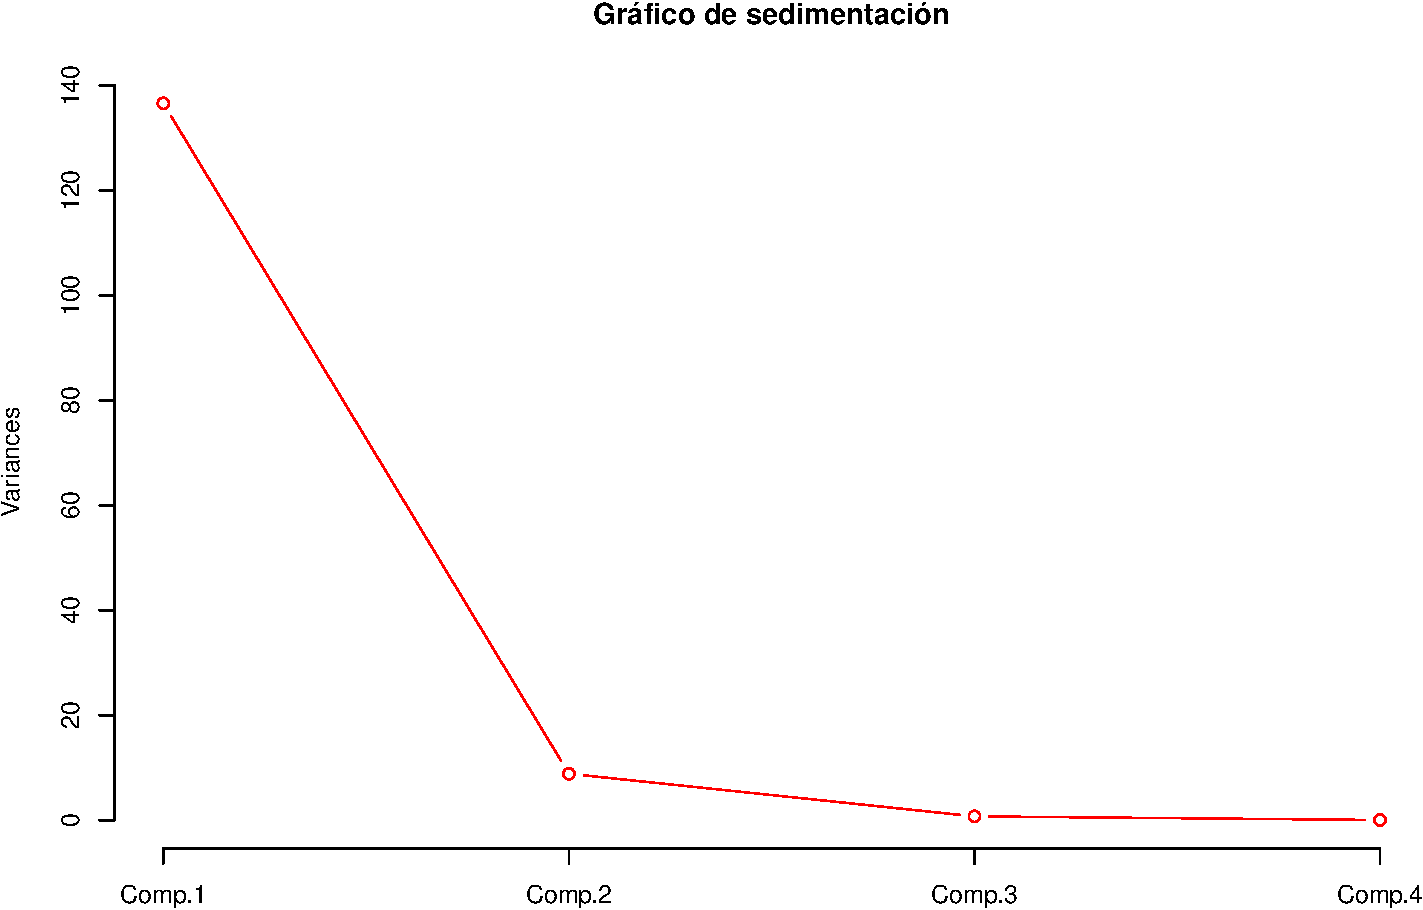
\includegraphics{AnalisisComponentesPrincipales_fusion_files/figure-beamer/screeplotlines-1.pdf}
\end{frame}

\begin{frame}{Gráfico de sedimentación, regla del codo, barras.}
\protect\hypertarget{gruxe1fico-de-sedimentaciuxf3n-regla-del-codo-barras.}{}
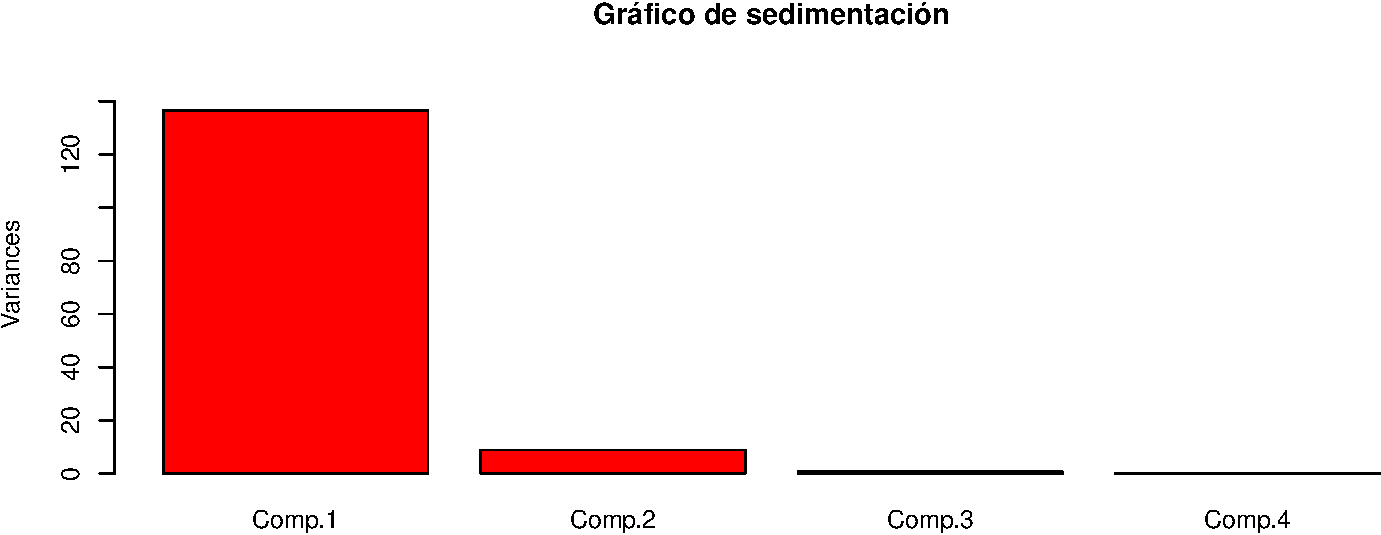
\includegraphics{AnalisisComponentesPrincipales_fusion_files/figure-beamer/screeplotbar-1.pdf}

Hay muchas otras pruebas más como la pruebas de Hipótesis de Anderson:

\[\left\{ \begin{array}{l}
H_0: \lambda_m=\ldots=\lambda_p\\ H_1: \mbox{no todos
iguales}\end{array}\right.\]
\end{frame}

\hypertarget{adecuaciuxf3n-de-los-datos-al-acp}{%
\section{Adecuación de los datos al
ACP}\label{adecuaciuxf3n-de-los-datos-al-acp}}

\begin{frame}{Adecuación de los datos al ACP}
\protect\hypertarget{adecuaciuxf3n-de-los-datos-al-acp-1}{}
\begin{itemize}
\tightlist
\item
  \red{Coeficiente de adecuación muestral (Kaiser Meyer y Olkin)}:
\end{itemize}

\[KMO=\frac{\sum_j \sum_{i\not =j} r_{i j}^2}{\sum_j \sum_{i\not =j} r^2_{i j}+
\sum_j \sum_{i\not =j} a^2_{i j}}\]

donde \(r_{i j}\) son los coef. de correlación entre las variables \(i\)
y \(j\), mientras que los \(a_{i j}\) son los coef. de correlación
parcial entre las variables \(i\) y \(j\) (equivalentes a las
correlaciones entre los residuos de la regresiones de estas dos
variables con las restantes).
\end{frame}

\begin{frame}[fragile]{Adecuación de los datos al ACP}
\protect\hypertarget{adecuaciuxf3n-de-los-datos-al-acp-2}{}
\begin{itemize}
\tightlist
\item
  Niveles de KMO \(\geq 0.5\) son considerados aceptables.
\end{itemize}

En nuestro ejemplo, las correlaciones parciales son:

\begin{Shaded}
\begin{Highlighting}[]
\FunctionTok{library}\NormalTok{(corpcor)}
\FunctionTok{cor2pcor}\NormalTok{(}\FunctionTok{cor}\NormalTok{(X))}
\end{Highlighting}
\end{Shaded}

\begin{verbatim}
##           [,1]       [,2]        [,3]        [,4]
## [1,] 1.0000000  0.9957943  0.90468746  0.31170534
## [2,] 0.9957943  1.0000000 -0.89188935 -0.31783572
## [3,] 0.9046875 -0.8918894  1.00000000  0.03389341
## [4,] 0.3117053 -0.3178357  0.03389341  1.00000000
\end{verbatim}
\end{frame}

\begin{frame}[fragile]{Adecuación de los datos al ACP}
\protect\hypertarget{adecuaciuxf3n-de-los-datos-al-acp-3}{}
Crearemos una funcióin que calcule el KMO:

\begin{Shaded}
\begin{Highlighting}[]
\NormalTok{kmo.test }\OtherTok{\textless{}{-}} \ControlFlowTok{function}\NormalTok{(df)\{}
\NormalTok{cor.sq }\OtherTok{=} \FunctionTok{cor}\NormalTok{(df)}\SpecialCharTok{\^{}}\DecValTok{2}
\NormalTok{cor.sumsq }\OtherTok{=}\NormalTok{ (}\FunctionTok{sum}\NormalTok{(cor.sq)}\SpecialCharTok{{-}}\FunctionTok{dim}\NormalTok{(cor.sq)[}\DecValTok{1}\NormalTok{])}
\NormalTok{pcor.sq }\OtherTok{=} \FunctionTok{cor2pcor}\NormalTok{(}\FunctionTok{cor}\NormalTok{(df))}\SpecialCharTok{\^{}}\DecValTok{2}
\NormalTok{pcor.sumsq }\OtherTok{=}\NormalTok{ (}\FunctionTok{sum}\NormalTok{(pcor.sq)}\SpecialCharTok{{-}}\FunctionTok{dim}\NormalTok{(pcor.sq)[}\DecValTok{1}\NormalTok{])}
\NormalTok{kmo }\OtherTok{=}\NormalTok{ cor.sumsq}\SpecialCharTok{/}\NormalTok{(cor.sumsq}\SpecialCharTok{+}\NormalTok{pcor.sumsq)}
\FunctionTok{return}\NormalTok{(kmo)}
\NormalTok{\} }

\FunctionTok{kmo.test}\NormalTok{(X)}
\end{Highlighting}
\end{Shaded}

\begin{verbatim}
## [1] 0.4225498
\end{verbatim}

El test esfericidad de Barlett contrasta si la matriz de correlaciones
es la identidad.

\[\left\{ \begin{array}{l}
H_0: \mbox{La matriz de correlaciones es la identidad}\\\\ H_1: \mbox{es
distinta de la
identidad}\end{array}\right.\]

Para que el ACP sea útil interesa rechazar la hipótesis nula, pues si
\(\mathbf{R}=I\) los componentes principales son las propias variables y
no se produce una reducción de los factores.

Este test, al igual que casi todas las propiedades de los estimadores en
ACP, requiere multinormalidad en la distribución de las variables.

En nuestro ejemplo:

\begin{Shaded}
\begin{Highlighting}[]
\FunctionTok{library}\NormalTok{(psych)}
\FunctionTok{cortest.bartlett}\NormalTok{(}\FunctionTok{cor}\NormalTok{(X),}\AttributeTok{n=}\NormalTok{n)}
\end{Highlighting}
\end{Shaded}

\begin{verbatim}
## $chisq
## [1] 35.89478
## 
## $p.value
## [1] 2.889513e-06
## 
## $df
## [1] 6
\end{verbatim}

El \(p\)-valor es muy pequeño por lo que no podemos aceptar la hipótesis
nula, la matriz de correlaciones es significativamente distinta de la
identidad.
\end{frame}

\hypertarget{descomposiciuxf3n-en-valores-singulares-svd}{%
\section{Descomposición en valores singulares
(SVD)}\label{descomposiciuxf3n-en-valores-singulares-svd}}

\begin{frame}{Descomposición en valores singulares}
\protect\hypertarget{descomposiciuxf3n-en-valores-singulares}{}
Dada un matriz de datos \(\mathbf{X}\) de dimensiones \(n\times p\),
donde \(n\geq p\) y de rango \(p\), se puede descomponer en producto de
tres matrices:

\[
\mathbf{X}=\mathbf{U}\cdot \Sigma\cdot \mathbf{V}^t, \mbox{ donde}
\]

\begin{itemize}
\tightlist
\item
  \(\mathbf{U}\) es una matriz ortogonal \(n\times p\) que tiene por
  columnas los \(p\) vectores propios de la matriz
  \(\mathbf{X}\mathbf{X}^t\) asociados a los \(p\) valores propios no
  nulos.
\item
  \({\Sigma}\) es una matriz diagonal \(p\times p\) que tiene por
  diagonal las raíces cuadradas de los valores propios de la matriz
  \(\mathbf{X}^t\mathbf{X}\).
\item
  \(\mathbf{V}\) es una matriz ortogonal \(p\times p\) que tiene por
  columnas los vectores propios de la matriz
  \(\mathbf{X}^t\cdot \mathbf{X}\) asociados a los \(p\) valores propios
  no nulos.
\end{itemize}
\end{frame}

\begin{frame}[fragile]{Descomposición en valores singulares (SVD):
ejemplo}
\protect\hypertarget{descomposiciuxf3n-en-valores-singulares-svd-ejemplo}{}
Consideramos la matriz \(\mathbf{X}\) como la matriz de datos centrada
del ejemplo de los niños.

\begin{verbatim}
##       [,1]       [,2]        [,3]       [,4]
##  [1,]   -3 -0.5777778 -0.88111111 -0.1333333
##  [2,]  -12 -3.2777778 -1.48111111 -3.3333333
##  [3,]   -4 -2.4777778  0.77888889  2.5666667
##  [4,]    7  0.2222222  1.88888889  6.8666667
##  [5,]  -14 -5.7777778 -0.42111111 -2.4333333
##  [6,]   -1 -0.7777778  0.68888889 -1.9333333
##  [7,]   -7 -0.7777778 -1.32111111 -1.3333333
##  [8,]   13  4.2222222  0.66888889  0.6666667
##  [9,]   21  9.2222222  0.07888889 -0.9333333
\end{verbatim}
\end{frame}

\begin{frame}{Descomposición en valores singulares (SVD): ejemplo}
\protect\hypertarget{descomposiciuxf3n-en-valores-singulares-svd-ejemplo-1}{}
La matriz \(\mathbf{X}^t\cdot \mathbf{X}\) vale:

\[
\mathbf{X}^t\cdot \mathbf{X}=\begin{pmatrix}
  1074.000 & 388.200 & 55.330 & 112.600 \\ 
  388.200 & 154.736 & 10.330 & 16.977 \\ 
  55.330 & 10.330 & 9.995 & 21.851 \\ 
  112.600 & 16.977 & 21.851 & 77.620 
\end{pmatrix}
\]
\end{frame}

\begin{frame}{Descomposición en valores singulares (SVD): ejemplo}
\protect\hypertarget{descomposiciuxf3n-en-valores-singulares-svd-ejemplo-2}{}
La matriz \(\mathbf{X}\cdot \mathbf{X}^t\) vale: (mostramos solo las 4
primeras columnas, la dimensión es \(9\times 9\))

\[
{\footnotesize
\mathbf{X}\cdot \mathbf{X}^t=\begin{pmatrix}
10.128 & 39.643 & 12.403 & -23.708 \\ 
  39.643 & 168.049 & 46.412 & -110.415 \\ 
  12.403 & 46.412 & 29.334 & -9.455 \\ 
  -23.708 & -110.415 & -9.455 & 99.768 \\ 
  46.034 & 195.673 & 63.742 & -116.788 \\ 
  3.100 & 19.974 & 1.502 & -19.147 \\ 
  22.791 & 92.951 & 25.476 & -60.824 \\ 
  -42.118 & -173.052 & -60.230 & 97.780 \\ 
  -68.273 & -279.234 & -109.185 & 142.790
\end{pmatrix}
}
\]
\end{frame}

\begin{frame}{Descomposición en valores singulares (SVD): ejemplo}
\protect\hypertarget{descomposiciuxf3n-en-valores-singulares-svd-ejemplo-3}{}
Los valores propios de la matriz \(\mathbf{X}^t\mathbf{X}\) son:

\[
\lambda_1=1229.538,\quad \lambda_2=79.751,\quad \lambda_3=6.641, \quad  
\lambda_4= 0.421. 
\]

Por lo tanto, la matriz \(\Sigma\) será:

\[
\Sigma =\begin{pmatrix} 
35.065 & 0.000 & 0.000 & 0.000 \\ 
  0.000 & 8.930 & 0.000 & 0.000 \\ 
  0.000 & 0.000 & 2.577 & 0.000 \\ 
  0.000 & 0.000 & 0.000 & 0.649 
  \end{pmatrix}
\]
\end{frame}

\begin{frame}{Descomposición en valores singulares (SVD): ejemplo}
\protect\hypertarget{descomposiciuxf3n-en-valores-singulares-svd-ejemplo-4}{}
La matriz \(\mathbf{U}\) será la siguiente la matriz \(10\times 4\) de
los vectores propios de los valores propios no nulos de \(X\cdot X^t\):

\[
\mathbf{U} =\begin{pmatrix}
-0.087 & 0.017 & 0.332 & 0.426 \\ 
  -0.362 & 0.279 & 0.129 & 0.159 \\ 
  -0.123 & -0.360 & -0.003 & -0.354 \\ 
  0.208 & -0.750 & 0.067 & 0.036 \\ 
  -0.436 & 0.076 & -0.420 & 0.294 \\ 
  -0.038 & 0.140 & -0.558 & -0.485 \\ 
  -0.199 & 0.153 & 0.577 & -0.370 \\ 
  0.391 & 0.022 & -0.203 & 0.434 \\ 
  0.647 & 0.424 & 0.079 & -0.140 
  \end{pmatrix}
\]
\end{frame}

\begin{frame}{Descomposición en valores singulares (SVD): ejemplo}
\protect\hypertarget{descomposiciuxf3n-en-valores-singulares-svd-ejemplo-5}{}
La matriz \(\mathbf{V}\) será la siguiente matriz \(4\times 4\) de los
valores propios de \(X^t\cdot X\) :

\[
\mathbf{V} =\begin{pmatrix}
0.934 & -0.022 & 0.256 & 0.247 \\ 
  0.339 & 0.354 & -0.661 & -0.568 \\ 
  0.047 & -0.248 & 0.566 & -0.785 \\ 
  0.097 & -0.902 & -0.421 & -0.013
  \end{pmatrix}
\] Comprobar que \(\mathbf{X}=\mathbf{U}\Sigma\mathbf{V}t\).
\end{frame}

\hypertarget{relaciuxf3n-acp-con-svd}{%
\section{Relación ACP con SVD}\label{relaciuxf3n-acp-con-svd}}

\begin{frame}{Relación ACP con SVD}
\protect\hypertarget{relaciuxf3n-acp-con-svd-1}{}
Consideramos una matriz de datos \(\mathbf{X}\) \(n\times p\) que puede
ser centrada (\red{ACP de covarianzas}) o tipificada
(\red{ACP de correlaciones}).

Si consideramos su \red{SVD},
\(\mathbf{X}=\mathbf{U}\Sigma\mathbf{V}t\), tenemos que las
\red{componentes principales}, \(\mathbf{Y}\), valen
\(\mathbf{CP}=\mathbf{U}\Sigma\).
\end{frame}

\begin{frame}{Relación ACP con SVD}
\protect\hypertarget{relaciuxf3n-acp-con-svd-2}{}
La prueba es muy sencilla. Recordamos que las componentes principales
son: \(\mathbf{CP}=\mathbf{X}\mathbf{V}\), donde \(\mathbf{V}\) era la
matriz de vectores propios de la matriz de covarianzas

\[\mathbf{S}=\frac{1}{n}\mathbf{X}^t\cdot \mathbf{X}.\]

Ahora bien, esta matriz coincidirá con la matriz de vectores propios de
la matriz \(\mathbf{X}t\mathbf{X}\) puesto que los vectores propios de
la matriz anterior y de la matriz de covarianzas \(\mathbf{S}\) son los
mismos.

Por lo tanto,

\[\mathbf{Y}=\mathbf{X}\mathbf{V}=\mathbf{U}\Sigma\mathbf{V}t\mathbf{V}=\mathbf{U}\Sigma,\]
puesto que la matriz \(\mathbf{V}\) es ortogonal.
\end{frame}

\begin{frame}{Relación ACP con SVD}
\protect\hypertarget{relaciuxf3n-acp-con-svd-3}{}
\blue{Teorema}

El producto escalar de dos \blue{filas} de la matriz de datos
\(\mathbf{X}\) coincide con el producto escalar de dos \blue{filas} de
la matriz de \red{componentes principales} \(\mathbf{Y}\).

\textbf{Prueba}

El producto escalar de dos filas de la matriz \(\mathbf{X}\) viene dada
por la matriz \(\mathbf{X}\cdot\mathbf{X}^t\) pero: \[
\mathbf{X}\cdot \mathbf{X}^t= \mathbf{Y}\cdot \mathbf{V}^t\cdot\mathbf{V}\cdot\mathbf{Y}^t=\mathbf{Y}\cdot\mathbf{Y}^t,
\] esta última matriz nos da el producto escalar de dos filas de la
matriz de \red{componentes principales}.
\end{frame}

\begin{frame}[fragile]{Ejemplo biplot}
\protect\hypertarget{ejemplo-biplot}{}
\begin{Shaded}
\begin{Highlighting}[]
\NormalTok{factoextra}\SpecialCharTok{::}\FunctionTok{fviz\_pca\_ind}\NormalTok{(solacp,}
             \AttributeTok{col.ind =} \StringTok{"cos2"}\NormalTok{, }
             \CommentTok{\# Colorpor calidad de }
             \CommentTok{\# la prepresentación}
             \AttributeTok{gradient.cols =}
                     \FunctionTok{c}\NormalTok{(}\StringTok{"\#00AFBB"}\NormalTok{, }
                       \StringTok{"\#E7B800"}\NormalTok{, }\StringTok{"\#FC4E07"}\NormalTok{),}
             \AttributeTok{repel =} \ConstantTok{TRUE}
             \CommentTok{\# permite  solapar texto}
\NormalTok{             )}
\end{Highlighting}
\end{Shaded}
\end{frame}

\begin{frame}{Ejemplo biplot}
\protect\hypertarget{ejemplo-biplot-1}{}
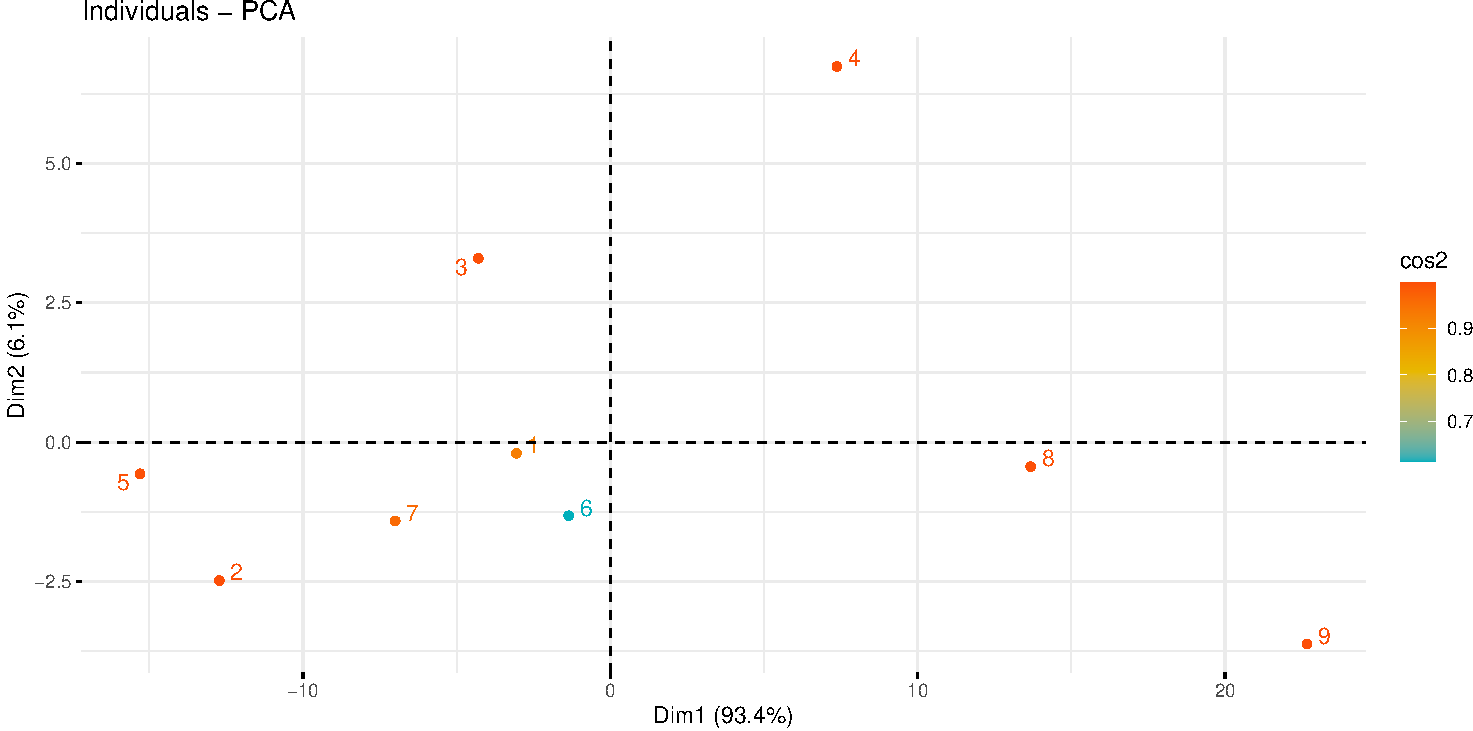
\includegraphics{AnalisisComponentesPrincipales_fusion_files/figure-beamer/biplot3-1.pdf}
\end{frame}

\begin{frame}{Interpretación de un biplot}
\protect\hypertarget{interpretaciuxf3n-de-un-biplot}{}
\begin{itemize}
\tightlist
\item
  La representación de las observaciones o los datos en un biplot
  equivale a proyectar las observaciones sobre el plano de las
  componentes principales estandarizadas para que tengan varianza
  unidad.
\item
  La representación de variables mediante vectores de dos coordenadas
  cumple que la correlación entre dos variables iniciales
  \(\mathbf{X}_i\) y \(\mathbf{X}_j\) es aproximadamente el coseno del
  ángulo que forman en el biplot. Por tanto, si dos variables
  \(\mathbf{X}_i\) y \(\mathbf{X}_j\) están muy correlacionadas, el
  coseno será grande y el ángulo entre los vectores, pequeño. En caso
  contrario, si están poco correlacionadas, el coseno será pequeño y el
  ángulo entre los vectores estará próximo a un ángulo recto.
\end{itemize}
\end{frame}

\begin{frame}{Comunalidades.}
\protect\hypertarget{comunalidades.}{}
En un ACP la comunalidad de la variable \(X_j\) retenida por las \(k\)
primeras componentes es la proporción de varianza de la variable que
queda explicada por esas componentes. Por ejemplo.

\begin{itemize}
\tightlist
\item
  Si retenemos sólo el componente \(CP_1\) la comunalidad de la variable
  \(X_j\) es:
\end{itemize}

\[h_j=r_{j 1}^2=\left( u_{1 j}\sqrt{\lambda_1}\right)^2\]

\begin{itemize}
\tightlist
\item
  Si retenemos los componentes\(CP_1\) y \(CP_2\) la comunalidad de la
  variable \(X_j\) es:
\end{itemize}

\[h_j=r_{j 1}^2+r_{2 j}^2=\left( u_{1 j}\sqrt{\lambda_1}\right)^2+
\left( u_{2 j}\sqrt{\lambda_2}\right)^2\]
\end{frame}

\hypertarget{interpretaciuxf3n-de-las-variables-y-los-individuos}{%
\section{Interpretación de las variables y los
individuos}\label{interpretaciuxf3n-de-las-variables-y-los-individuos}}

\begin{frame}{Interpretación de las variables y los individuos}
\protect\hypertarget{interpretaciuxf3n-de-las-variables-y-los-individuos-1}{}
\begin{itemize}
\item
  Las variables también pueden representar de forma simultanea con los
  individuos en los componentes principales.
\item
  Esta representación se hace mediante las coordenadas que la matriz de
  componentes que nos explican las correlaciones de cada factor con cada
  variable.
\end{itemize}
\end{frame}

\begin{frame}{Circulo de correlación}
\protect\hypertarget{circulo-de-correlaciuxf3n}{}
\begin{itemize}
\tightlist
\item
  Cada variable está representada por el vector que une el origen de
  coordenadas cono el punto.
\item
  Todos están en círculo unidad (círculo de correlación).
\item
  A medida que cada variable se acerca a la circunferencia unidad está
  mejor representado por los componentes retenidas y viceversa.
\item
  El ángulo entre variables y componentes nos da una idea de su
  correlación, al nivel de retención de varianza total que tengamos.
\item
  Así variable perpendiculares tenderán a ser \emph{incorreladas}.
\item
  Los valores de una variable crecen en la dirección de ésta.
\end{itemize}
\end{frame}

\begin{frame}[fragile]{Circulo de correlación}
\protect\hypertarget{circulo-de-correlaciuxf3n-1}{}
\begin{Shaded}
\begin{Highlighting}[]
\NormalTok{factoextra}\SpecialCharTok{::}\FunctionTok{fviz\_pca\_var}\NormalTok{(solacp,}
             \AttributeTok{col.var =} \StringTok{"contrib"}\NormalTok{,}
             \CommentTok{\# Color por contribución asl pca}
             \AttributeTok{gradient.cols =} \FunctionTok{c}\NormalTok{(}\StringTok{"\#00AFBB"}\NormalTok{,}
                               \StringTok{"\#E7B800"}\NormalTok{,}
                               \StringTok{"\#FC4E07"}\NormalTok{),}
             \AttributeTok{repel =} \ConstantTok{TRUE}    
\NormalTok{             )}
\end{Highlighting}
\end{Shaded}
\end{frame}

\begin{frame}{Circulo de correlación}
\protect\hypertarget{circulo-de-correlaciuxf3n-2}{}
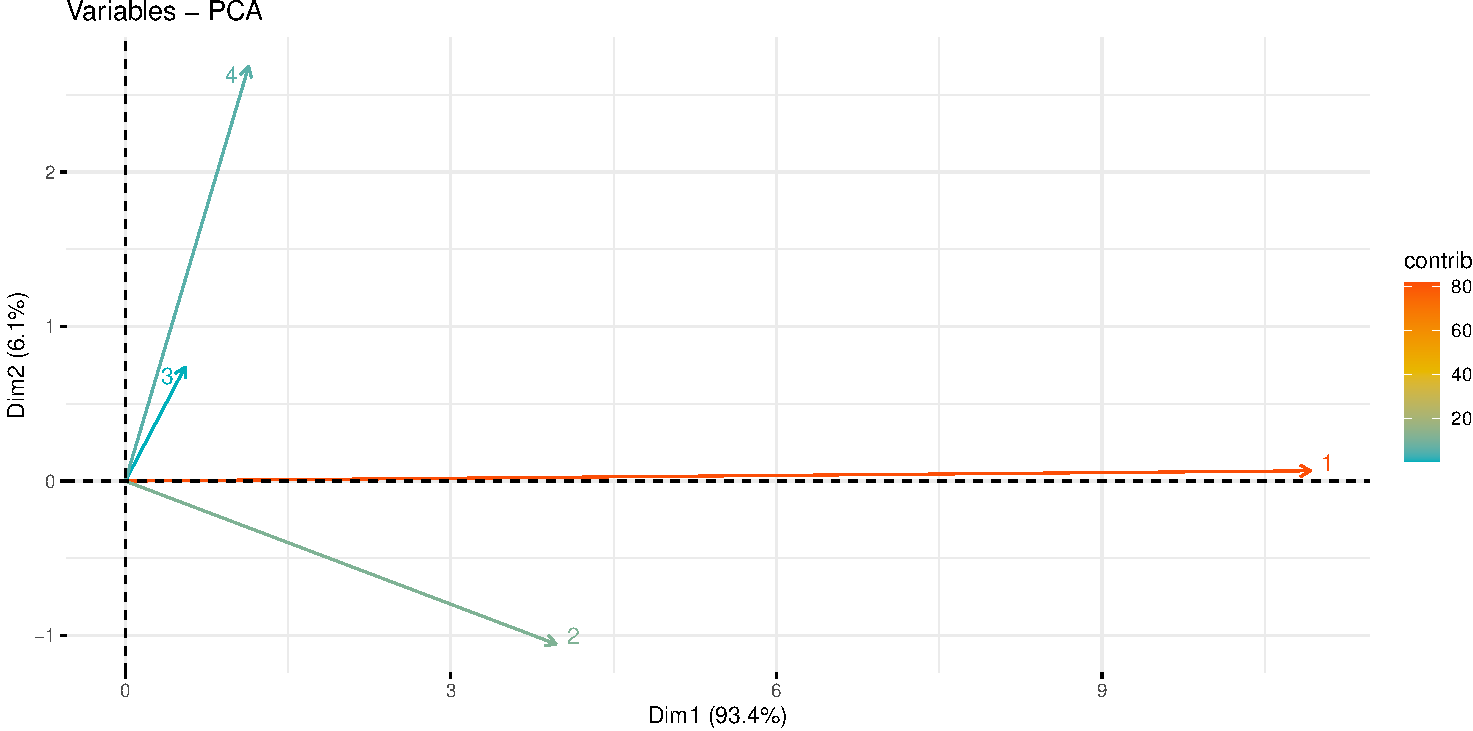
\includegraphics{AnalisisComponentesPrincipales_fusion_files/figure-beamer/biplor-1.pdf}
\end{frame}

\hypertarget{y-muchas-cosas-muxe1s..}{%
\section{Y muchas cosas más..}\label{y-muchas-cosas-muxe1s..}}

\begin{frame}{Y muchas cosas más..}
\protect\hypertarget{y-muchas-cosas-muxe1s..-1}{}
Para acabar\ldots{}
\blue{Análisis Factorial Confirmatorio yExploratorio}

\begin{itemize}
\item
  El Análisis factorial confirmatorio se realiza sobre modelos
  establecidos de factores y se hacen inferencias sobre sus propiedades.
\item
  El análisis factorial descriptivo ayuda a la descripción de los datos
  y a la búsqueda de factores.
\end{itemize}

\blue{Relación del ACP con otras técnicas de análisis de datos}

\begin{itemize}
\tightlist
\item
  Regresión Lineal Múltiple
\item
  Clasificación.
\item
  Análisis de correspondencias simples y múltiples.
\item
  \ldots{} y muchas otras más
\end{itemize}
\end{frame}

\end{document}
